\documentclass[11pt]{article}

    \usepackage[breakable]{tcolorbox}
    \usepackage{parskip} % Stop auto-indenting (to mimic markdown behaviour)
    
    \usepackage{iftex}
    \ifPDFTeX
    	\usepackage[T1]{fontenc}
    	\usepackage{mathpazo}
    \else
    	\usepackage{fontspec}
    \fi

    % Basic figure setup, for now with no caption control since it's done
    % automatically by Pandoc (which extracts ![](path) syntax from Markdown).
    \usepackage{graphicx}
    % Maintain compatibility with old templates. Remove in nbconvert 6.0
    \let\Oldincludegraphics\includegraphics
    % Ensure that by default, figures have no caption (until we provide a
    % proper Figure object with a Caption API and a way to capture that
    % in the conversion process - todo).
    \usepackage{caption}
    \DeclareCaptionFormat{nocaption}{}
    \captionsetup{format=nocaption,aboveskip=0pt,belowskip=0pt}

    \usepackage{float}
    \floatplacement{figure}{H} % forces figures to be placed at the correct location
    \usepackage{xcolor} % Allow colors to be defined
    \usepackage{enumerate} % Needed for markdown enumerations to work
    \usepackage{geometry} % Used to adjust the document margins
    \usepackage{amsmath} % Equations
    \usepackage{amssymb} % Equations
    \usepackage{textcomp} % defines textquotesingle
    % Hack from http://tex.stackexchange.com/a/47451/13684:
    \AtBeginDocument{%
        \def\PYZsq{\textquotesingle}% Upright quotes in Pygmentized code
    }
    \usepackage{upquote} % Upright quotes for verbatim code
    \usepackage{eurosym} % defines \euro
    \usepackage[mathletters]{ucs} % Extended unicode (utf-8) support
    \usepackage{fancyvrb} % verbatim replacement that allows latex
    \usepackage{grffile} % extends the file name processing of package graphics 
                         % to support a larger range
    \makeatletter % fix for old versions of grffile with XeLaTeX
    \@ifpackagelater{grffile}{2019/11/01}
    {
      % Do nothing on new versions
    }
    {
      \def\Gread@@xetex#1{%
        \IfFileExists{"\Gin@base".bb}%
        {\Gread@eps{\Gin@base.bb}}%
        {\Gread@@xetex@aux#1}%
      }
    }
    \makeatother
    \usepackage[Export]{adjustbox} % Used to constrain images to a maximum size
    \adjustboxset{max size={0.9\linewidth}{0.9\paperheight}}

    % The hyperref package gives us a pdf with properly built
    % internal navigation ('pdf bookmarks' for the table of contents,
    % internal cross-reference links, web links for URLs, etc.)
    \usepackage{hyperref}
    % The default LaTeX title has an obnoxious amount of whitespace. By default,
    % titling removes some of it. It also provides customization options.
    \usepackage{titling}
    \usepackage{longtable} % longtable support required by pandoc >1.10
    \usepackage{booktabs}  % table support for pandoc > 1.12.2
    \usepackage[inline]{enumitem} % IRkernel/repr support (it uses the enumerate* environment)
    \usepackage[normalem]{ulem} % ulem is needed to support strikethroughs (\sout)
                                % normalem makes italics be italics, not underlines
    \usepackage{mathrsfs}
    

    
    % Colors for the hyperref package
    \definecolor{urlcolor}{rgb}{0,.145,.698}
    \definecolor{linkcolor}{rgb}{.71,0.21,0.01}
    \definecolor{citecolor}{rgb}{.12,.54,.11}

    % ANSI colors
    \definecolor{ansi-black}{HTML}{3E424D}
    \definecolor{ansi-black-intense}{HTML}{282C36}
    \definecolor{ansi-red}{HTML}{E75C58}
    \definecolor{ansi-red-intense}{HTML}{B22B31}
    \definecolor{ansi-green}{HTML}{00A250}
    \definecolor{ansi-green-intense}{HTML}{007427}
    \definecolor{ansi-yellow}{HTML}{DDB62B}
    \definecolor{ansi-yellow-intense}{HTML}{B27D12}
    \definecolor{ansi-blue}{HTML}{208FFB}
    \definecolor{ansi-blue-intense}{HTML}{0065CA}
    \definecolor{ansi-magenta}{HTML}{D160C4}
    \definecolor{ansi-magenta-intense}{HTML}{A03196}
    \definecolor{ansi-cyan}{HTML}{60C6C8}
    \definecolor{ansi-cyan-intense}{HTML}{258F8F}
    \definecolor{ansi-white}{HTML}{C5C1B4}
    \definecolor{ansi-white-intense}{HTML}{A1A6B2}
    \definecolor{ansi-default-inverse-fg}{HTML}{FFFFFF}
    \definecolor{ansi-default-inverse-bg}{HTML}{000000}

    % common color for the border for error outputs.
    \definecolor{outerrorbackground}{HTML}{FFDFDF}

    % commands and environments needed by pandoc snippets
    % extracted from the output of `pandoc -s`
    \providecommand{\tightlist}{%
      \setlength{\itemsep}{0pt}\setlength{\parskip}{0pt}}
    \DefineVerbatimEnvironment{Highlighting}{Verbatim}{commandchars=\\\{\}}
    % Add ',fontsize=\small' for more characters per line
    \newenvironment{Shaded}{}{}
    \newcommand{\KeywordTok}[1]{\textcolor[rgb]{0.00,0.44,0.13}{\textbf{{#1}}}}
    \newcommand{\DataTypeTok}[1]{\textcolor[rgb]{0.56,0.13,0.00}{{#1}}}
    \newcommand{\DecValTok}[1]{\textcolor[rgb]{0.25,0.63,0.44}{{#1}}}
    \newcommand{\BaseNTok}[1]{\textcolor[rgb]{0.25,0.63,0.44}{{#1}}}
    \newcommand{\FloatTok}[1]{\textcolor[rgb]{0.25,0.63,0.44}{{#1}}}
    \newcommand{\CharTok}[1]{\textcolor[rgb]{0.25,0.44,0.63}{{#1}}}
    \newcommand{\StringTok}[1]{\textcolor[rgb]{0.25,0.44,0.63}{{#1}}}
    \newcommand{\CommentTok}[1]{\textcolor[rgb]{0.38,0.63,0.69}{\textit{{#1}}}}
    \newcommand{\OtherTok}[1]{\textcolor[rgb]{0.00,0.44,0.13}{{#1}}}
    \newcommand{\AlertTok}[1]{\textcolor[rgb]{1.00,0.00,0.00}{\textbf{{#1}}}}
    \newcommand{\FunctionTok}[1]{\textcolor[rgb]{0.02,0.16,0.49}{{#1}}}
    \newcommand{\RegionMarkerTok}[1]{{#1}}
    \newcommand{\ErrorTok}[1]{\textcolor[rgb]{1.00,0.00,0.00}{\textbf{{#1}}}}
    \newcommand{\NormalTok}[1]{{#1}}
    
    % Additional commands for more recent versions of Pandoc
    \newcommand{\ConstantTok}[1]{\textcolor[rgb]{0.53,0.00,0.00}{{#1}}}
    \newcommand{\SpecialCharTok}[1]{\textcolor[rgb]{0.25,0.44,0.63}{{#1}}}
    \newcommand{\VerbatimStringTok}[1]{\textcolor[rgb]{0.25,0.44,0.63}{{#1}}}
    \newcommand{\SpecialStringTok}[1]{\textcolor[rgb]{0.73,0.40,0.53}{{#1}}}
    \newcommand{\ImportTok}[1]{{#1}}
    \newcommand{\DocumentationTok}[1]{\textcolor[rgb]{0.73,0.13,0.13}{\textit{{#1}}}}
    \newcommand{\AnnotationTok}[1]{\textcolor[rgb]{0.38,0.63,0.69}{\textbf{\textit{{#1}}}}}
    \newcommand{\CommentVarTok}[1]{\textcolor[rgb]{0.38,0.63,0.69}{\textbf{\textit{{#1}}}}}
    \newcommand{\VariableTok}[1]{\textcolor[rgb]{0.10,0.09,0.49}{{#1}}}
    \newcommand{\ControlFlowTok}[1]{\textcolor[rgb]{0.00,0.44,0.13}{\textbf{{#1}}}}
    \newcommand{\OperatorTok}[1]{\textcolor[rgb]{0.40,0.40,0.40}{{#1}}}
    \newcommand{\BuiltInTok}[1]{{#1}}
    \newcommand{\ExtensionTok}[1]{{#1}}
    \newcommand{\PreprocessorTok}[1]{\textcolor[rgb]{0.74,0.48,0.00}{{#1}}}
    \newcommand{\AttributeTok}[1]{\textcolor[rgb]{0.49,0.56,0.16}{{#1}}}
    \newcommand{\InformationTok}[1]{\textcolor[rgb]{0.38,0.63,0.69}{\textbf{\textit{{#1}}}}}
    \newcommand{\WarningTok}[1]{\textcolor[rgb]{0.38,0.63,0.69}{\textbf{\textit{{#1}}}}}
    
    
    % Define a nice break command that doesn't care if a line doesn't already
    % exist.
    \def\br{\hspace*{\fill} \\* }
    % Math Jax compatibility definitions
    \def\gt{>}
    \def\lt{<}
    \let\Oldtex\TeX
    \let\Oldlatex\LaTeX
    \renewcommand{\TeX}{\textrm{\Oldtex}}
    \renewcommand{\LaTeX}{\textrm{\Oldlatex}}
    % Document parameters
    % Document title
    \title{Arrays}
    
    
    
    
    
% Pygments definitions
\makeatletter
\def\PY@reset{\let\PY@it=\relax \let\PY@bf=\relax%
    \let\PY@ul=\relax \let\PY@tc=\relax%
    \let\PY@bc=\relax \let\PY@ff=\relax}
\def\PY@tok#1{\csname PY@tok@#1\endcsname}
\def\PY@toks#1+{\ifx\relax#1\empty\else%
    \PY@tok{#1}\expandafter\PY@toks\fi}
\def\PY@do#1{\PY@bc{\PY@tc{\PY@ul{%
    \PY@it{\PY@bf{\PY@ff{#1}}}}}}}
\def\PY#1#2{\PY@reset\PY@toks#1+\relax+\PY@do{#2}}

\@namedef{PY@tok@w}{\def\PY@tc##1{\textcolor[rgb]{0.73,0.73,0.73}{##1}}}
\@namedef{PY@tok@c}{\let\PY@it=\textit\def\PY@tc##1{\textcolor[rgb]{0.25,0.50,0.50}{##1}}}
\@namedef{PY@tok@cp}{\def\PY@tc##1{\textcolor[rgb]{0.74,0.48,0.00}{##1}}}
\@namedef{PY@tok@k}{\let\PY@bf=\textbf\def\PY@tc##1{\textcolor[rgb]{0.00,0.50,0.00}{##1}}}
\@namedef{PY@tok@kp}{\def\PY@tc##1{\textcolor[rgb]{0.00,0.50,0.00}{##1}}}
\@namedef{PY@tok@kt}{\def\PY@tc##1{\textcolor[rgb]{0.69,0.00,0.25}{##1}}}
\@namedef{PY@tok@o}{\def\PY@tc##1{\textcolor[rgb]{0.40,0.40,0.40}{##1}}}
\@namedef{PY@tok@ow}{\let\PY@bf=\textbf\def\PY@tc##1{\textcolor[rgb]{0.67,0.13,1.00}{##1}}}
\@namedef{PY@tok@nb}{\def\PY@tc##1{\textcolor[rgb]{0.00,0.50,0.00}{##1}}}
\@namedef{PY@tok@nf}{\def\PY@tc##1{\textcolor[rgb]{0.00,0.00,1.00}{##1}}}
\@namedef{PY@tok@nc}{\let\PY@bf=\textbf\def\PY@tc##1{\textcolor[rgb]{0.00,0.00,1.00}{##1}}}
\@namedef{PY@tok@nn}{\let\PY@bf=\textbf\def\PY@tc##1{\textcolor[rgb]{0.00,0.00,1.00}{##1}}}
\@namedef{PY@tok@ne}{\let\PY@bf=\textbf\def\PY@tc##1{\textcolor[rgb]{0.82,0.25,0.23}{##1}}}
\@namedef{PY@tok@nv}{\def\PY@tc##1{\textcolor[rgb]{0.10,0.09,0.49}{##1}}}
\@namedef{PY@tok@no}{\def\PY@tc##1{\textcolor[rgb]{0.53,0.00,0.00}{##1}}}
\@namedef{PY@tok@nl}{\def\PY@tc##1{\textcolor[rgb]{0.63,0.63,0.00}{##1}}}
\@namedef{PY@tok@ni}{\let\PY@bf=\textbf\def\PY@tc##1{\textcolor[rgb]{0.60,0.60,0.60}{##1}}}
\@namedef{PY@tok@na}{\def\PY@tc##1{\textcolor[rgb]{0.49,0.56,0.16}{##1}}}
\@namedef{PY@tok@nt}{\let\PY@bf=\textbf\def\PY@tc##1{\textcolor[rgb]{0.00,0.50,0.00}{##1}}}
\@namedef{PY@tok@nd}{\def\PY@tc##1{\textcolor[rgb]{0.67,0.13,1.00}{##1}}}
\@namedef{PY@tok@s}{\def\PY@tc##1{\textcolor[rgb]{0.73,0.13,0.13}{##1}}}
\@namedef{PY@tok@sd}{\let\PY@it=\textit\def\PY@tc##1{\textcolor[rgb]{0.73,0.13,0.13}{##1}}}
\@namedef{PY@tok@si}{\let\PY@bf=\textbf\def\PY@tc##1{\textcolor[rgb]{0.73,0.40,0.53}{##1}}}
\@namedef{PY@tok@se}{\let\PY@bf=\textbf\def\PY@tc##1{\textcolor[rgb]{0.73,0.40,0.13}{##1}}}
\@namedef{PY@tok@sr}{\def\PY@tc##1{\textcolor[rgb]{0.73,0.40,0.53}{##1}}}
\@namedef{PY@tok@ss}{\def\PY@tc##1{\textcolor[rgb]{0.10,0.09,0.49}{##1}}}
\@namedef{PY@tok@sx}{\def\PY@tc##1{\textcolor[rgb]{0.00,0.50,0.00}{##1}}}
\@namedef{PY@tok@m}{\def\PY@tc##1{\textcolor[rgb]{0.40,0.40,0.40}{##1}}}
\@namedef{PY@tok@gh}{\let\PY@bf=\textbf\def\PY@tc##1{\textcolor[rgb]{0.00,0.00,0.50}{##1}}}
\@namedef{PY@tok@gu}{\let\PY@bf=\textbf\def\PY@tc##1{\textcolor[rgb]{0.50,0.00,0.50}{##1}}}
\@namedef{PY@tok@gd}{\def\PY@tc##1{\textcolor[rgb]{0.63,0.00,0.00}{##1}}}
\@namedef{PY@tok@gi}{\def\PY@tc##1{\textcolor[rgb]{0.00,0.63,0.00}{##1}}}
\@namedef{PY@tok@gr}{\def\PY@tc##1{\textcolor[rgb]{1.00,0.00,0.00}{##1}}}
\@namedef{PY@tok@ge}{\let\PY@it=\textit}
\@namedef{PY@tok@gs}{\let\PY@bf=\textbf}
\@namedef{PY@tok@gp}{\let\PY@bf=\textbf\def\PY@tc##1{\textcolor[rgb]{0.00,0.00,0.50}{##1}}}
\@namedef{PY@tok@go}{\def\PY@tc##1{\textcolor[rgb]{0.53,0.53,0.53}{##1}}}
\@namedef{PY@tok@gt}{\def\PY@tc##1{\textcolor[rgb]{0.00,0.27,0.87}{##1}}}
\@namedef{PY@tok@err}{\def\PY@bc##1{{\setlength{\fboxsep}{\string -\fboxrule}\fcolorbox[rgb]{1.00,0.00,0.00}{1,1,1}{\strut ##1}}}}
\@namedef{PY@tok@kc}{\let\PY@bf=\textbf\def\PY@tc##1{\textcolor[rgb]{0.00,0.50,0.00}{##1}}}
\@namedef{PY@tok@kd}{\let\PY@bf=\textbf\def\PY@tc##1{\textcolor[rgb]{0.00,0.50,0.00}{##1}}}
\@namedef{PY@tok@kn}{\let\PY@bf=\textbf\def\PY@tc##1{\textcolor[rgb]{0.00,0.50,0.00}{##1}}}
\@namedef{PY@tok@kr}{\let\PY@bf=\textbf\def\PY@tc##1{\textcolor[rgb]{0.00,0.50,0.00}{##1}}}
\@namedef{PY@tok@bp}{\def\PY@tc##1{\textcolor[rgb]{0.00,0.50,0.00}{##1}}}
\@namedef{PY@tok@fm}{\def\PY@tc##1{\textcolor[rgb]{0.00,0.00,1.00}{##1}}}
\@namedef{PY@tok@vc}{\def\PY@tc##1{\textcolor[rgb]{0.10,0.09,0.49}{##1}}}
\@namedef{PY@tok@vg}{\def\PY@tc##1{\textcolor[rgb]{0.10,0.09,0.49}{##1}}}
\@namedef{PY@tok@vi}{\def\PY@tc##1{\textcolor[rgb]{0.10,0.09,0.49}{##1}}}
\@namedef{PY@tok@vm}{\def\PY@tc##1{\textcolor[rgb]{0.10,0.09,0.49}{##1}}}
\@namedef{PY@tok@sa}{\def\PY@tc##1{\textcolor[rgb]{0.73,0.13,0.13}{##1}}}
\@namedef{PY@tok@sb}{\def\PY@tc##1{\textcolor[rgb]{0.73,0.13,0.13}{##1}}}
\@namedef{PY@tok@sc}{\def\PY@tc##1{\textcolor[rgb]{0.73,0.13,0.13}{##1}}}
\@namedef{PY@tok@dl}{\def\PY@tc##1{\textcolor[rgb]{0.73,0.13,0.13}{##1}}}
\@namedef{PY@tok@s2}{\def\PY@tc##1{\textcolor[rgb]{0.73,0.13,0.13}{##1}}}
\@namedef{PY@tok@sh}{\def\PY@tc##1{\textcolor[rgb]{0.73,0.13,0.13}{##1}}}
\@namedef{PY@tok@s1}{\def\PY@tc##1{\textcolor[rgb]{0.73,0.13,0.13}{##1}}}
\@namedef{PY@tok@mb}{\def\PY@tc##1{\textcolor[rgb]{0.40,0.40,0.40}{##1}}}
\@namedef{PY@tok@mf}{\def\PY@tc##1{\textcolor[rgb]{0.40,0.40,0.40}{##1}}}
\@namedef{PY@tok@mh}{\def\PY@tc##1{\textcolor[rgb]{0.40,0.40,0.40}{##1}}}
\@namedef{PY@tok@mi}{\def\PY@tc##1{\textcolor[rgb]{0.40,0.40,0.40}{##1}}}
\@namedef{PY@tok@il}{\def\PY@tc##1{\textcolor[rgb]{0.40,0.40,0.40}{##1}}}
\@namedef{PY@tok@mo}{\def\PY@tc##1{\textcolor[rgb]{0.40,0.40,0.40}{##1}}}
\@namedef{PY@tok@ch}{\let\PY@it=\textit\def\PY@tc##1{\textcolor[rgb]{0.25,0.50,0.50}{##1}}}
\@namedef{PY@tok@cm}{\let\PY@it=\textit\def\PY@tc##1{\textcolor[rgb]{0.25,0.50,0.50}{##1}}}
\@namedef{PY@tok@cpf}{\let\PY@it=\textit\def\PY@tc##1{\textcolor[rgb]{0.25,0.50,0.50}{##1}}}
\@namedef{PY@tok@c1}{\let\PY@it=\textit\def\PY@tc##1{\textcolor[rgb]{0.25,0.50,0.50}{##1}}}
\@namedef{PY@tok@cs}{\let\PY@it=\textit\def\PY@tc##1{\textcolor[rgb]{0.25,0.50,0.50}{##1}}}

\def\PYZbs{\char`\\}
\def\PYZus{\char`\_}
\def\PYZob{\char`\{}
\def\PYZcb{\char`\}}
\def\PYZca{\char`\^}
\def\PYZam{\char`\&}
\def\PYZlt{\char`\<}
\def\PYZgt{\char`\>}
\def\PYZsh{\char`\#}
\def\PYZpc{\char`\%}
\def\PYZdl{\char`\$}
\def\PYZhy{\char`\-}
\def\PYZsq{\char`\'}
\def\PYZdq{\char`\"}
\def\PYZti{\char`\~}
% for compatibility with earlier versions
\def\PYZat{@}
\def\PYZlb{[}
\def\PYZrb{]}
\makeatother


    % For linebreaks inside Verbatim environment from package fancyvrb. 
    \makeatletter
        \newbox\Wrappedcontinuationbox 
        \newbox\Wrappedvisiblespacebox 
        \newcommand*\Wrappedvisiblespace {\textcolor{red}{\textvisiblespace}} 
        \newcommand*\Wrappedcontinuationsymbol {\textcolor{red}{\llap{\tiny$\m@th\hookrightarrow$}}} 
        \newcommand*\Wrappedcontinuationindent {3ex } 
        \newcommand*\Wrappedafterbreak {\kern\Wrappedcontinuationindent\copy\Wrappedcontinuationbox} 
        % Take advantage of the already applied Pygments mark-up to insert 
        % potential linebreaks for TeX processing. 
        %        {, <, #, %, $, ' and ": go to next line. 
        %        _, }, ^, &, >, - and ~: stay at end of broken line. 
        % Use of \textquotesingle for straight quote. 
        \newcommand*\Wrappedbreaksatspecials {% 
            \def\PYGZus{\discretionary{\char`\_}{\Wrappedafterbreak}{\char`\_}}% 
            \def\PYGZob{\discretionary{}{\Wrappedafterbreak\char`\{}{\char`\{}}% 
            \def\PYGZcb{\discretionary{\char`\}}{\Wrappedafterbreak}{\char`\}}}% 
            \def\PYGZca{\discretionary{\char`\^}{\Wrappedafterbreak}{\char`\^}}% 
            \def\PYGZam{\discretionary{\char`\&}{\Wrappedafterbreak}{\char`\&}}% 
            \def\PYGZlt{\discretionary{}{\Wrappedafterbreak\char`\<}{\char`\<}}% 
            \def\PYGZgt{\discretionary{\char`\>}{\Wrappedafterbreak}{\char`\>}}% 
            \def\PYGZsh{\discretionary{}{\Wrappedafterbreak\char`\#}{\char`\#}}% 
            \def\PYGZpc{\discretionary{}{\Wrappedafterbreak\char`\%}{\char`\%}}% 
            \def\PYGZdl{\discretionary{}{\Wrappedafterbreak\char`\$}{\char`\$}}% 
            \def\PYGZhy{\discretionary{\char`\-}{\Wrappedafterbreak}{\char`\-}}% 
            \def\PYGZsq{\discretionary{}{\Wrappedafterbreak\textquotesingle}{\textquotesingle}}% 
            \def\PYGZdq{\discretionary{}{\Wrappedafterbreak\char`\"}{\char`\"}}% 
            \def\PYGZti{\discretionary{\char`\~}{\Wrappedafterbreak}{\char`\~}}% 
        } 
        % Some characters . , ; ? ! / are not pygmentized. 
        % This macro makes them "active" and they will insert potential linebreaks 
        \newcommand*\Wrappedbreaksatpunct {% 
            \lccode`\~`\.\lowercase{\def~}{\discretionary{\hbox{\char`\.}}{\Wrappedafterbreak}{\hbox{\char`\.}}}% 
            \lccode`\~`\,\lowercase{\def~}{\discretionary{\hbox{\char`\,}}{\Wrappedafterbreak}{\hbox{\char`\,}}}% 
            \lccode`\~`\;\lowercase{\def~}{\discretionary{\hbox{\char`\;}}{\Wrappedafterbreak}{\hbox{\char`\;}}}% 
            \lccode`\~`\:\lowercase{\def~}{\discretionary{\hbox{\char`\:}}{\Wrappedafterbreak}{\hbox{\char`\:}}}% 
            \lccode`\~`\?\lowercase{\def~}{\discretionary{\hbox{\char`\?}}{\Wrappedafterbreak}{\hbox{\char`\?}}}% 
            \lccode`\~`\!\lowercase{\def~}{\discretionary{\hbox{\char`\!}}{\Wrappedafterbreak}{\hbox{\char`\!}}}% 
            \lccode`\~`\/\lowercase{\def~}{\discretionary{\hbox{\char`\/}}{\Wrappedafterbreak}{\hbox{\char`\/}}}% 
            \catcode`\.\active
            \catcode`\,\active 
            \catcode`\;\active
            \catcode`\:\active
            \catcode`\?\active
            \catcode`\!\active
            \catcode`\/\active 
            \lccode`\~`\~ 	
        }
    \makeatother

    \let\OriginalVerbatim=\Verbatim
    \makeatletter
    \renewcommand{\Verbatim}[1][1]{%
        %\parskip\z@skip
        \sbox\Wrappedcontinuationbox {\Wrappedcontinuationsymbol}%
        \sbox\Wrappedvisiblespacebox {\FV@SetupFont\Wrappedvisiblespace}%
        \def\FancyVerbFormatLine ##1{\hsize\linewidth
            \vtop{\raggedright\hyphenpenalty\z@\exhyphenpenalty\z@
                \doublehyphendemerits\z@\finalhyphendemerits\z@
                \strut ##1\strut}%
        }%
        % If the linebreak is at a space, the latter will be displayed as visible
        % space at end of first line, and a continuation symbol starts next line.
        % Stretch/shrink are however usually zero for typewriter font.
        \def\FV@Space {%
            \nobreak\hskip\z@ plus\fontdimen3\font minus\fontdimen4\font
            \discretionary{\copy\Wrappedvisiblespacebox}{\Wrappedafterbreak}
            {\kern\fontdimen2\font}%
        }%
        
        % Allow breaks at special characters using \PYG... macros.
        \Wrappedbreaksatspecials
        % Breaks at punctuation characters . , ; ? ! and / need catcode=\active 	
        \OriginalVerbatim[#1,codes*=\Wrappedbreaksatpunct]%
    }
    \makeatother

    % Exact colors from NB
    \definecolor{incolor}{HTML}{303F9F}
    \definecolor{outcolor}{HTML}{D84315}
    \definecolor{cellborder}{HTML}{CFCFCF}
    \definecolor{cellbackground}{HTML}{F7F7F7}
    
    % prompt
    \makeatletter
    \newcommand{\boxspacing}{\kern\kvtcb@left@rule\kern\kvtcb@boxsep}
    \makeatother
    \newcommand{\prompt}[4]{
        {\ttfamily\llap{{\color{#2}[#3]:\hspace{3pt}#4}}\vspace{-\baselineskip}}
    }
    

    
    % Prevent overflowing lines due to hard-to-break entities
    \sloppy 
    % Setup hyperref package
    \hypersetup{
      breaklinks=true,  % so long urls are correctly broken across lines
      colorlinks=true,
      urlcolor=urlcolor,
      linkcolor=linkcolor,
      citecolor=citecolor,
      }
    % Slightly bigger margins than the latex defaults
    
    \geometry{verbose,tmargin=1in,bmargin=1in,lmargin=1in,rmargin=1in}
    
    

\begin{document}
    
    \maketitle
    
    

    
    \hypertarget{arrays}{%
\section{Arrays}\label{arrays}}

\hypertarget{topics}{%
\subsection{Topics}\label{topics}}

\begin{itemize}
\tightlist
\item
  C-array introduction
\item
  static and dynamic arrays
\item
  similarity between arrays and pointers
\item
  passing arrays to functions
\item
  aggregate operations on arrays
\item
  C-string - array of characters
\item
  buffer overflow security flaw
\item
  sorting data
\item
  2-d array and tic-tac-toe game
\end{itemize}

    \hypertarget{array}{%
\subsection{Array}\label{array}}

\begin{itemize}
\tightlist
\item
  dictionary defintion of array is a range of a particular type of thing
\item
  we've used single variable to store single data/value
\item
  large programs typically deal with a large number of data values that
  must be stored in memory e.g.~sorting data values.
\item
  NOT practicle to declare a large number of variables to store a large
  number of values
\item
  array is a container used to store a large number of same type values
  under one name
\item
  array we're learning about in this chapter is C-array
\item
  since C++11 standard, C++ provides \textbf{array} and \textbf{vector}
  types under STL (standard template library)

  \begin{itemize}
  \tightlist
  \item
    these advanced types (array and vector) are similar to C++ string
    type
  \end{itemize}
\item
  understanding the C-array helps understand many C++ concepts and data
  structures that rely on C-array

  \begin{itemize}
  \tightlist
  \item
    plus, a large no. of legacy C++ codebase and libraries specially
    developed before C++11 may be still using C-array
  \end{itemize}
\item
  C++ vector is a better choice among C++ \textbf{array} and C-array, if
  your comipler supports it

  \begin{itemize}
  \tightlist
  \item
    vector takes care of all the common operations one would do in an
    array
  \item
    similar to C-string (more below) vs C++ string
  \end{itemize}
\item
  array in this notebook refers to C-array
\item
  there are two types of array:

  \begin{enumerate}
  \def\labelenumi{\arabic{enumi}.}
  \tightlist
  \item
    static array
  \item
    dynamic array
  \end{enumerate}
\end{itemize}

\hypertarget{static-array}{%
\subsection{Static array}\label{static-array}}

\begin{itemize}
\tightlist
\item
  the size of the array is determined during compile-time and is fixed
\item
  local static array is stored on stack memory segment
\item
  syntax to declare a static array
\end{itemize}

\begin{Shaded}
\begin{Highlighting}[]
\NormalTok{type arrayName}\OperatorTok{[}\NormalTok{size}\OperatorTok{];}
\end{Highlighting}
\end{Shaded}

\begin{itemize}
\tightlist
\item
  \texttt{size} tells the compiler how many of similar type of values
  can be stored in the arrayName
\item
  \texttt{size} must be a positive integer (size\_t type) - literal or
  variable
\item
  the following figure depicts computer memory when an array of
  \texttt{int} is declared
\end{itemize}

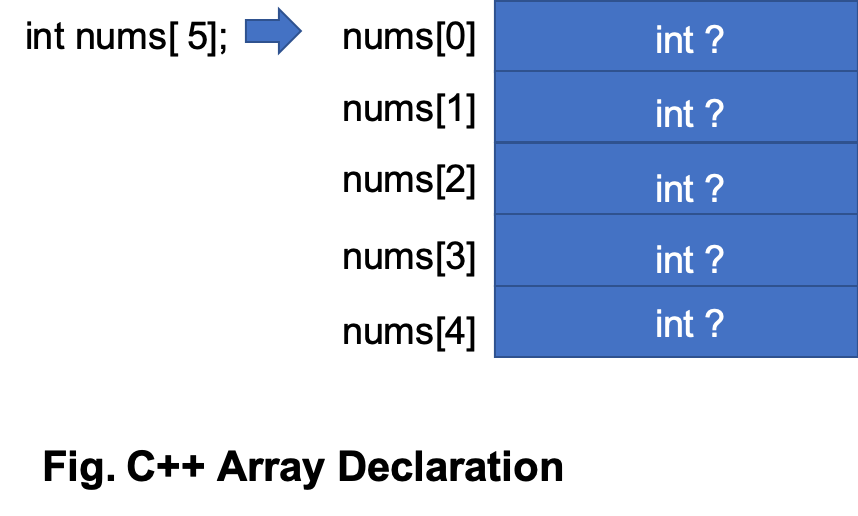
\includegraphics{resources/array.png}

\begin{itemize}
\tightlist
\item
  each member of the array is called an element
\item
  each element has same type and share same array name but different
  index
\item
  index also called offset ranges between 0 to size-1
\end{itemize}

\hypertarget{visualize-array-using-pythontutor.com}{%
\subsubsection{\texorpdfstring{Visualize array using
\href{http://pythontutor.com/cpp.html\#code=//\%20pass\%20by\%20value\%20demo\%0A\%23include\%20\%3Ciostream\%3E\%0Ausing\%20namespace\%20std\%3B\%0A\%0Aint\%20main\%28\%29\%20\%7B\%0A\%20\%20int\%20nums\%5B5\%5D\%3B\%0A\%20\%20nums\%5B0\%5D\%20\%3D\%2010\%3B\%0A\%20\%20nums\%5B1\%5D\%20\%3D\%2020\%3B\%0A\%20\%20nums\%5B2\%5D\%20\%3D\%2030\%3B\%0A\%20\%20nums\%5B3\%5D\%20\%3D\%2040\%3B\%0A\%20\%20nums\%5B4\%5D\%20\%3D\%2050\%3B\%0A\%20\%20nums\%5B1\%5D\%20\%3D\%20nums\%5B2\%5D\%20\%2B\%20nums\%5B3\%5D\%3B\%0A\%20\%20for\%28int\%20i\%3D0\%3B\%20i\%3C5\%3B\%20i\%2B\%2B\%29\%0A\%20\%20\%20\%20cout\%20\%3C\%3C\%20nums\%5Bi\%5D\%20\%3C\%3C\%20endl\%3B\%0A\%20\%20return\%200\%3B\%0A\%7D\&curInstr=0\&mode=display\&origin=opt-frontend.js\&py=cpp\&rawInputLstJSON=\%5B\%5D}{pythontutor.com}}{Visualize array using pythontutor.com}}\label{visualize-array-using-pythontutor.com}}

    \begin{tcolorbox}[breakable, size=fbox, boxrule=1pt, pad at break*=1mm,colback=cellbackground, colframe=cellborder]
\prompt{In}{incolor}{1}{\boxspacing}
\begin{Verbatim}[commandchars=\\\{\}]
\PY{c+cp}{\PYZsh{}}\PY{c+cp}{include} \PY{c+cpf}{\PYZlt{}iostream\PYZgt{}}
\PY{c+cp}{\PYZsh{}}\PY{c+cp}{include} \PY{c+cpf}{\PYZlt{}string\PYZgt{}}

\PY{k}{using} \PY{k}{namespace} \PY{n+nn}{std}\PY{p}{;}
\end{Verbatim}
\end{tcolorbox}

    \begin{tcolorbox}[breakable, size=fbox, boxrule=1pt, pad at break*=1mm,colback=cellbackground, colframe=cellborder]
\prompt{In}{incolor}{2}{\boxspacing}
\begin{Verbatim}[commandchars=\\\{\}]
\PY{c+c1}{// nums array to store 5 integers}
\PY{k+kt}{int} \PY{n}{nums}\PY{p}{[}\PY{l+m+mi}{5}\PY{p}{]}\PY{p}{;}
\end{Verbatim}
\end{tcolorbox}

    \hypertarget{accessing-member-elements}{%
\subsubsection{Accessing member
elements}\label{accessing-member-elements}}

\begin{itemize}
\tightlist
\item
  members can be accessed and used ONLY one element per operation
\item
  no aggregate operation is allowed on the array variable as a whole

  \begin{itemize}
  \tightlist
  \item
    e.g.~copy one array into another; printing the whole array, etc.
  \item
    only aggregate operation allowed is during array initialization
  \end{itemize}
\end{itemize}

    \begin{tcolorbox}[breakable, size=fbox, boxrule=1pt, pad at break*=1mm,colback=cellbackground, colframe=cellborder]
\prompt{In}{incolor}{3}{\boxspacing}
\begin{Verbatim}[commandchars=\\\{\}]
\PY{c+c1}{// access and store values into each element}
\PY{n}{nums}\PY{p}{[}\PY{l+m+mi}{0}\PY{p}{]} \PY{o}{=} \PY{l+m+mi}{10}\PY{p}{;}
\PY{n}{nums}\PY{p}{[}\PY{l+m+mi}{1}\PY{p}{]} \PY{o}{=} \PY{l+m+mi}{20}\PY{p}{;}
\PY{n}{nums}\PY{p}{[}\PY{l+m+mi}{2}\PY{p}{]} \PY{o}{=} \PY{l+m+mi}{30}\PY{p}{;}
\PY{n}{nums}\PY{p}{[}\PY{l+m+mi}{3}\PY{p}{]} \PY{o}{=} \PY{l+m+mi}{40}\PY{p}{;}
\PY{n}{nums}\PY{p}{[}\PY{l+m+mi}{4}\PY{p}{]} \PY{o}{=} \PY{l+m+mi}{50}\PY{p}{;}
\end{Verbatim}
\end{tcolorbox}

    \begin{tcolorbox}[breakable, size=fbox, boxrule=1pt, pad at break*=1mm,colback=cellbackground, colframe=cellborder]
\prompt{In}{incolor}{4}{\boxspacing}
\begin{Verbatim}[commandchars=\\\{\}]
\PY{c+c1}{// access some element}
\PY{n}{cout} \PY{o}{\PYZlt{}}\PY{o}{\PYZlt{}} \PY{n}{nums}\PY{p}{[}\PY{l+m+mi}{0}\PY{p}{]}\PY{p}{;}
\end{Verbatim}
\end{tcolorbox}

    \begin{Verbatim}[commandchars=\\\{\}]
10
    \end{Verbatim}

    \begin{tcolorbox}[breakable, size=fbox, boxrule=1pt, pad at break*=1mm,colback=cellbackground, colframe=cellborder]
\prompt{In}{incolor}{5}{\boxspacing}
\begin{Verbatim}[commandchars=\\\{\}]
\PY{c+c1}{// each element can be used like a single variable}
\PY{n}{nums}\PY{p}{[}\PY{l+m+mi}{1}\PY{p}{]} \PY{o}{=} \PY{n}{nums}\PY{p}{[}\PY{l+m+mi}{2}\PY{p}{]} \PY{o}{+} \PY{n}{nums}\PY{p}{[}\PY{l+m+mi}{3}\PY{p}{]}\PY{p}{;}
\end{Verbatim}
\end{tcolorbox}

    \begin{tcolorbox}[breakable, size=fbox, boxrule=1pt, pad at break*=1mm,colback=cellbackground, colframe=cellborder]
\prompt{In}{incolor}{6}{\boxspacing}
\begin{Verbatim}[commandchars=\\\{\}]
\PY{c+c1}{// traverse an array}
\PY{k}{for}\PY{p}{(}\PY{k+kt}{int} \PY{n}{i}\PY{o}{=}\PY{l+m+mi}{0}\PY{p}{;} \PY{n}{i}\PY{o}{\PYZlt{}}\PY{l+m+mi}{5}\PY{p}{;} \PY{n}{i}\PY{o}{+}\PY{o}{+}\PY{p}{)} \PY{p}{\PYZob{}}
    \PY{n}{cout} \PY{o}{\PYZlt{}}\PY{o}{\PYZlt{}} \PY{n}{i} \PY{o}{\PYZlt{}}\PY{o}{\PYZlt{}} \PY{l+s}{\PYZdq{}}\PY{l+s}{ \PYZhy{}\PYZgt{} }\PY{l+s}{\PYZdq{}} \PY{o}{\PYZlt{}}\PY{o}{\PYZlt{}} \PY{n}{nums}\PY{p}{[}\PY{n}{i}\PY{p}{]} \PY{o}{\PYZlt{}}\PY{o}{\PYZlt{}} \PY{n}{endl}\PY{p}{;}
\PY{p}{\PYZcb{}}
\end{Verbatim}
\end{tcolorbox}

    \begin{Verbatim}[commandchars=\\\{\}]
0 -> 10
1 -> 70
2 -> 30
3 -> 40
4 -> 50
    \end{Verbatim}

    \begin{tcolorbox}[breakable, size=fbox, boxrule=1pt, pad at break*=1mm,colback=cellbackground, colframe=cellborder]
\prompt{In}{incolor}{7}{\boxspacing}
\begin{Verbatim}[commandchars=\\\{\}]
\PY{c+c1}{// declaring and initializing an array}
\PY{c+c1}{// size is optinal; will be determined with the no. of values it\PYZsq{}s initialzed with}
\PY{k+kt}{float} \PY{n}{grades}\PY{p}{[}\PY{p}{]} \PY{o}{=} \PY{p}{\PYZob{}}\PY{l+m+mf}{90.5f}\PY{p}{,} \PY{l+m+mf}{34.5f}\PY{p}{,} \PY{l+m+mi}{56}\PY{p}{,} \PY{l+m+mi}{81}\PY{p}{,} \PY{l+m+mi}{99}\PY{p}{,} \PY{l+m+mi}{100}\PY{p}{,} \PY{l+m+mf}{89.9}\PY{p}{\PYZcb{}}\PY{p}{;}
\end{Verbatim}
\end{tcolorbox}

    \begin{tcolorbox}[breakable, size=fbox, boxrule=1pt, pad at break*=1mm,colback=cellbackground, colframe=cellborder]
\prompt{In}{incolor}{8}{\boxspacing}
\begin{Verbatim}[commandchars=\\\{\}]
\PY{n}{grades}
\end{Verbatim}
\end{tcolorbox}

            \begin{tcolorbox}[breakable, size=fbox, boxrule=.5pt, pad at break*=1mm, opacityfill=0]
\prompt{Out}{outcolor}{8}{\boxspacing}
\begin{Verbatim}[commandchars=\\\{\}]
\{ 90.5000f, 34.5000f, 56.0000f, 81.0000f, 99.0000f, 100.000f, 89.9000f \}
\end{Verbatim}
\end{tcolorbox}
        
    \hypertarget{member-functions}{%
\subsection{Member functions}\label{member-functions}}

\begin{itemize}
\tightlist
\item
  C-array is so primitive that it doesn't come with any useful
  operations or member functions
\item
  implementing any array operation falls under programmer's
  responsibility!
\item
  e.g.~how can you quickly tell the size or length of an array?
\end{itemize}

    \begin{tcolorbox}[breakable, size=fbox, boxrule=1pt, pad at break*=1mm,colback=cellbackground, colframe=cellborder]
\prompt{In}{incolor}{9}{\boxspacing}
\begin{Verbatim}[commandchars=\\\{\}]
\PY{c+c1}{// finding the size of the array}
\PY{k+kt}{size\PYZus{}t} \PY{n}{arr\PYZus{}size} \PY{o}{=} \PY{k}{sizeof}\PY{p}{(}\PY{n}{grades}\PY{p}{)}\PY{o}{/}\PY{k+kt}{float}\PY{p}{(}\PY{k}{sizeof}\PY{p}{(}\PY{k+kt}{float}\PY{p}{)}\PY{p}{)}\PY{p}{;}
\end{Verbatim}
\end{tcolorbox}

    \begin{tcolorbox}[breakable, size=fbox, boxrule=1pt, pad at break*=1mm,colback=cellbackground, colframe=cellborder]
\prompt{In}{incolor}{10}{\boxspacing}
\begin{Verbatim}[commandchars=\\\{\}]
\PY{n}{cout} \PY{o}{\PYZlt{}}\PY{o}{\PYZlt{}} \PY{l+s}{\PYZdq{}}\PY{l+s}{array\PYZsq{}s size or length = }\PY{l+s}{\PYZdq{}} \PY{o}{\PYZlt{}}\PY{o}{\PYZlt{}} \PY{n}{arr\PYZus{}size}\PY{p}{;}
\end{Verbatim}
\end{tcolorbox}

    \begin{Verbatim}[commandchars=\\\{\}]
array's size or length = 7
    \end{Verbatim}

    \begin{tcolorbox}[breakable, size=fbox, boxrule=1pt, pad at break*=1mm,colback=cellbackground, colframe=cellborder]
\prompt{In}{incolor}{11}{\boxspacing}
\begin{Verbatim}[commandchars=\\\{\}]
\PY{n}{cout} \PY{o}{\PYZlt{}}\PY{o}{\PYZlt{}} \PY{l+s}{\PYZdq{}}\PY{l+s}{last grade = }\PY{l+s}{\PYZdq{}} \PY{o}{\PYZlt{}}\PY{o}{\PYZlt{}} \PY{n}{grades}\PY{p}{[}\PY{n}{arr\PYZus{}size}\PY{l+m+mi}{\PYZhy{}1}\PY{p}{]} \PY{o}{\PYZlt{}}\PY{o}{\PYZlt{}} \PY{n}{endl}\PY{p}{;}
\end{Verbatim}
\end{tcolorbox}

    \begin{Verbatim}[commandchars=\\\{\}]
last grade = 89.9
    \end{Verbatim}

    \hypertarget{array-size-is-fixed}{%
\subsubsection{Array size is fixed!}\label{array-size-is-fixed}}

\begin{itemize}
\tightlist
\item
  one has to know how many elements will be stored in a given array
\item
  what happens when the array is full?
\end{itemize}

    \begin{tcolorbox}[breakable, size=fbox, boxrule=1pt, pad at break*=1mm,colback=cellbackground, colframe=cellborder]
\prompt{In}{incolor}{12}{\boxspacing}
\begin{Verbatim}[commandchars=\\\{\}]
\PY{c+c1}{// grades doesn\PYZsq{}t have index 7 as the size is 7}
\PY{n}{grades}\PY{p}{[}\PY{l+m+mi}{7}\PY{p}{]} \PY{o}{=} \PY{l+m+mi}{67}\PY{p}{;}
\end{Verbatim}
\end{tcolorbox}

    \begin{Verbatim}[commandchars=\\\{\}]
\textbf{input\_line\_22:3:1: }\textcolor{ansi-magenta-intense}{\textbf{warning: }}\textbf{array index 7 is past the
end of the array (which contains 7 elements) [-Warray-bounds]}
grades[7] = 67;
\textcolor{ansi-green-intense}{\textbf{\^{}      \textasciitilde{}
}}\textbf{input\_line\_14:4:1: }\textcolor{ansi-black-intense}{\textbf{note: }}array 'grades' declared
here
float grades[] = \{90.5f, 34.5f, 56, 81, 99, 100, 89.9\};
\textcolor{ansi-green-intense}{\textbf{\^{}
}}
    \end{Verbatim}

    \hypertarget{array-and-pointers}{%
\subsection{Array and Pointers}\label{array-and-pointers}}

\begin{itemize}
\tightlist
\item
  there's a lot of similarities on how array and pointers work!

  \begin{itemize}
  \tightlist
  \item
    they can be used interchangebly as desired
  \end{itemize}
\end{itemize}

    \begin{tcolorbox}[breakable, size=fbox, boxrule=1pt, pad at break*=1mm,colback=cellbackground, colframe=cellborder]
\prompt{In}{incolor}{13}{\boxspacing}
\begin{Verbatim}[commandchars=\\\{\}]
\PY{k+kt}{int} \PY{n}{ids}\PY{p}{[}\PY{p}{]} \PY{o}{=} \PY{p}{\PYZob{}}\PY{l+m+mi}{100}\PY{p}{,} \PY{l+m+mi}{200}\PY{p}{,} \PY{l+m+mi}{300}\PY{p}{,} \PY{l+m+mi}{400}\PY{p}{\PYZcb{}}\PY{p}{;}
\end{Verbatim}
\end{tcolorbox}

    \begin{tcolorbox}[breakable, size=fbox, boxrule=1pt, pad at break*=1mm,colback=cellbackground, colframe=cellborder]
\prompt{In}{incolor}{14}{\boxspacing}
\begin{Verbatim}[commandchars=\\\{\}]
\PY{c+c1}{// copy the base address of array}
\PY{c+c1}{// which is the address of element at index 0; which is \PYZam{}ids[0];}
\PY{k+kt}{int} \PY{o}{*} \PY{n}{ptr} \PY{o}{=} \PY{n}{ids}\PY{p}{;}
\end{Verbatim}
\end{tcolorbox}

    \begin{tcolorbox}[breakable, size=fbox, boxrule=1pt, pad at break*=1mm,colback=cellbackground, colframe=cellborder]
\prompt{In}{incolor}{15}{\boxspacing}
\begin{Verbatim}[commandchars=\\\{\}]
\PY{c+c1}{// print the base memory addresses}
\PY{n}{cout} \PY{o}{\PYZlt{}}\PY{o}{\PYZlt{}} \PY{n}{ptr} \PY{o}{\PYZlt{}}\PY{o}{\PYZlt{}} \PY{l+s}{\PYZdq{}}\PY{l+s}{ equals to }\PY{l+s}{\PYZdq{}} \PY{o}{\PYZlt{}}\PY{o}{\PYZlt{}} \PY{o}{\PYZam{}}\PY{n}{ids}\PY{p}{[}\PY{l+m+mi}{0}\PY{p}{]} \PY{o}{\PYZlt{}}\PY{o}{\PYZlt{}} \PY{l+s}{\PYZdq{}}\PY{l+s}{ equals to }\PY{l+s}{\PYZdq{}} \PY{o}{\PYZlt{}}\PY{o}{\PYZlt{}} \PY{n}{ids}\PY{p}{;}
\end{Verbatim}
\end{tcolorbox}

    \begin{Verbatim}[commandchars=\\\{\}]
0x109deff80 equals to 0x109deff80 equals to 0x109deff80
    \end{Verbatim}

    \begin{tcolorbox}[breakable, size=fbox, boxrule=1pt, pad at break*=1mm,colback=cellbackground, colframe=cellborder]
\prompt{In}{incolor}{16}{\boxspacing}
\begin{Verbatim}[commandchars=\\\{\}]
\PY{c+c1}{// print the data located at the base memory addresses}
\PY{n}{cout} \PY{o}{\PYZlt{}}\PY{o}{\PYZlt{}} \PY{o}{*}\PY{n}{ptr} \PY{o}{\PYZlt{}}\PY{o}{\PYZlt{}} \PY{l+s}{\PYZdq{}}\PY{l+s}{ equals to }\PY{l+s}{\PYZdq{}} \PY{o}{\PYZlt{}}\PY{o}{\PYZlt{}} \PY{n}{ids}\PY{p}{[}\PY{l+m+mi}{0}\PY{p}{]} \PY{o}{\PYZlt{}}\PY{o}{\PYZlt{}} \PY{l+s}{\PYZdq{}}\PY{l+s}{ equals to }\PY{l+s}{\PYZdq{}} \PY{o}{\PYZlt{}}\PY{o}{\PYZlt{}} \PY{o}{*}\PY{n}{ids}\PY{p}{;}
\end{Verbatim}
\end{tcolorbox}

    \begin{Verbatim}[commandchars=\\\{\}]
100 equals to 100 equals to 100
    \end{Verbatim}

    \begin{tcolorbox}[breakable, size=fbox, boxrule=1pt, pad at break*=1mm,colback=cellbackground, colframe=cellborder]
\prompt{In}{incolor}{17}{\boxspacing}
\begin{Verbatim}[commandchars=\\\{\}]
\PY{c+c1}{// using pointers to traverse array}
\PY{c+c1}{// point to the second element}
\PY{n}{ptr}\PY{o}{+}\PY{o}{+}\PY{p}{;}
\end{Verbatim}
\end{tcolorbox}

    \begin{tcolorbox}[breakable, size=fbox, boxrule=1pt, pad at break*=1mm,colback=cellbackground, colframe=cellborder]
\prompt{In}{incolor}{18}{\boxspacing}
\begin{Verbatim}[commandchars=\\\{\}]
\PY{c+c1}{// dereference the value at that location}
\PY{n}{cout} \PY{o}{\PYZlt{}}\PY{o}{\PYZlt{}} \PY{o}{*}\PY{n}{ptr} \PY{o}{\PYZlt{}}\PY{o}{\PYZlt{}} \PY{n}{endl}\PY{p}{;}
\end{Verbatim}
\end{tcolorbox}

    \begin{Verbatim}[commandchars=\\\{\}]
200
    \end{Verbatim}

    \begin{tcolorbox}[breakable, size=fbox, boxrule=1pt, pad at break*=1mm,colback=cellbackground, colframe=cellborder]
\prompt{In}{incolor}{19}{\boxspacing}
\begin{Verbatim}[commandchars=\\\{\}]
\PY{n}{ptr} \PY{o}{=} \PY{n}{ids}\PY{p}{;} \PY{c+c1}{// copy the base address}
\PY{k}{for}\PY{p}{(}\PY{k+kt}{int} \PY{n}{i}\PY{o}{=}\PY{l+m+mi}{0}\PY{p}{;} \PY{n}{i}\PY{o}{\PYZlt{}}\PY{l+m+mi}{4}\PY{p}{;} \PY{n}{i}\PY{o}{+}\PY{o}{+}\PY{p}{)} \PY{p}{\PYZob{}}
    \PY{n}{cout} \PY{o}{\PYZlt{}}\PY{o}{\PYZlt{}} \PY{n}{i} \PY{o}{\PYZlt{}}\PY{o}{\PYZlt{}} \PY{l+s}{\PYZdq{}}\PY{l+s}{\PYZhy{}\PYZgt{} }\PY{l+s}{\PYZdq{}} \PY{o}{\PYZlt{}}\PY{o}{\PYZlt{}} \PY{o}{*}\PY{p}{(}\PY{n}{ptr}\PY{o}{+}\PY{n}{i}\PY{p}{)} \PY{o}{\PYZlt{}}\PY{o}{\PYZlt{}} \PY{l+s}{\PYZdq{}}\PY{l+s}{ == }\PY{l+s}{\PYZdq{}} \PY{o}{\PYZlt{}}\PY{o}{\PYZlt{}} \PY{n}{ptr}\PY{p}{[}\PY{n}{i}\PY{p}{]} \PY{o}{\PYZlt{}}\PY{o}{\PYZlt{}} \PY{l+s}{\PYZdq{}}\PY{l+s}{ == }\PY{l+s}{\PYZdq{}} \PY{o}{\PYZlt{}}\PY{o}{\PYZlt{}} \PY{n}{ids}\PY{p}{[}\PY{n}{i}\PY{p}{]} \PY{o}{\PYZlt{}}\PY{o}{\PYZlt{}} \PY{n}{endl}\PY{p}{;}
\PY{p}{\PYZcb{}}
\end{Verbatim}
\end{tcolorbox}

    \begin{Verbatim}[commandchars=\\\{\}]
0-> 100 == 100 == 100
1-> 200 == 200 == 200
2-> 300 == 300 == 300
3-> 400 == 400 == 400
    \end{Verbatim}

    \hypertarget{dynamic-array}{%
\subsection{Dynamic array}\label{dynamic-array}}

\begin{itemize}
\tightlist
\item
  array size can be determined during run time (program execution)

  \begin{itemize}
  \tightlist
  \item
    once the size is set, it's fixed
  \end{itemize}
\item
  local dynamic array is allocated on the heap memory segment using
  pointer and \textbf{new} operator
\item
  syntax to declare dynamic array:
\end{itemize}

\begin{Shaded}
\begin{Highlighting}[]
\NormalTok{type }\OperatorTok{*}\NormalTok{ arrayName }\OperatorTok{=} \KeywordTok{new}\NormalTok{ type}\OperatorTok{[}\NormalTok{size}\OperatorTok{];}
\end{Highlighting}
\end{Shaded}

\begin{itemize}
\tightlist
\item
  size can be a variable determined or assigned during program execution
\item
  once the dynamic array is declared, using dynamic array is same as
  using static array
\item
  dynamic memory must be deallocated to prevent memory leak
\item
  syntax:
\end{itemize}

\begin{verbatim}
delete[] arrayName;
\end{verbatim}

\hypertarget{visualize-dynamic-array-in-pythontutor.com}{%
\subsubsection{\texorpdfstring{Visualize dynamic array in
\href{http://pythontutor.com/cpp.html\#code=//\%20pass\%20by\%20value\%20demo\%0A\%23include\%20\%3Ciostream\%3E\%0Ausing\%20namespace\%20std\%3B\%0A\%0Aint\%20main\%28\%29\%20\%7B\%0A\%20\%20size_t\%20arr_size\%20\%3D\%205\%3B\%0A\%20\%20int\%20*\%20nums\%20\%3D\%20new\%20int\%5Barr_size\%5D\%3B\%0A\%20\%20nums\%5B0\%5D\%20\%3D\%2010\%3B\%0A\%20\%20nums\%5B1\%5D\%20\%3D\%2020\%3B\%0A\%20\%20nums\%5B2\%5D\%20\%3D\%2030\%3B\%0A\%20\%20nums\%5B3\%5D\%20\%3D\%2040\%3B\%0A\%20\%20nums\%5B4\%5D\%20\%3D\%2050\%3B\%0A\%20\%20nums\%5B1\%5D\%20\%3D\%20nums\%5B2\%5D\%20\%2B\%20nums\%5B3\%5D\%3B\%0A\%20\%20for\%28int\%20i\%3D0\%3B\%20i\%3C5\%3B\%20i\%2B\%2B\%29\%0A\%20\%20\%20\%20cout\%20\%3C\%3C\%20nums\%5Bi\%5D\%20\%3C\%3C\%20endl\%3B\%0A\%20\%20\%0A\%20\%20delete\%5B\%5D\%20nums\%3B\%0A\%20\%20return\%200\%3B\%0A\%7D\&curInstr=0\&mode=display\&origin=opt-frontend.js\&py=cpp\&rawInputLstJSON=\%5B\%5D}{pythontutor.com}}{Visualize dynamic array in pythontutor.com}}\label{visualize-dynamic-array-in-pythontutor.com}}

    \begin{tcolorbox}[breakable, size=fbox, boxrule=1pt, pad at break*=1mm,colback=cellbackground, colframe=cellborder]
\prompt{In}{incolor}{20}{\boxspacing}
\begin{Verbatim}[commandchars=\\\{\}]
\PY{k+kt}{size\PYZus{}t} \PY{n}{capacity}\PY{p}{;}
\end{Verbatim}
\end{tcolorbox}

    \begin{tcolorbox}[breakable, size=fbox, boxrule=1pt, pad at break*=1mm,colback=cellbackground, colframe=cellborder]
\prompt{In}{incolor}{21}{\boxspacing}
\begin{Verbatim}[commandchars=\\\{\}]
\PY{n}{cout} \PY{o}{\PYZlt{}}\PY{o}{\PYZlt{}} \PY{l+s}{\PYZdq{}}\PY{l+s}{How many integers would you like to enter? }\PY{l+s}{\PYZdq{}}\PY{p}{;}
\PY{n}{cin} \PY{o}{\PYZgt{}}\PY{o}{\PYZgt{}} \PY{n}{capacity}\PY{p}{;}
\end{Verbatim}
\end{tcolorbox}

    \begin{Verbatim}[commandchars=\\\{\}]
How many integers would you like to enter?


3
    \end{Verbatim}

    \begin{tcolorbox}[breakable, size=fbox, boxrule=1pt, pad at break*=1mm,colback=cellbackground, colframe=cellborder]
\prompt{In}{incolor}{22}{\boxspacing}
\begin{Verbatim}[commandchars=\\\{\}]
\PY{k+kt}{int} \PY{o}{*} \PY{n}{some\PYZus{}array} \PY{o}{=} \PY{k}{new} \PY{k+kt}{int}\PY{p}{[}\PY{n}{capacity}\PY{p}{]}\PY{p}{;}
\end{Verbatim}
\end{tcolorbox}

    \begin{tcolorbox}[breakable, size=fbox, boxrule=1pt, pad at break*=1mm,colback=cellbackground, colframe=cellborder]
\prompt{In}{incolor}{23}{\boxspacing}
\begin{Verbatim}[commandchars=\\\{\}]
\PY{c+c1}{// prompt user to store capacity number of integers and store them into array}
\PY{k}{for}\PY{p}{(}\PY{k+kt}{int} \PY{n}{i}\PY{o}{=}\PY{l+m+mi}{0}\PY{p}{;} \PY{n}{i}\PY{o}{\PYZlt{}}\PY{n}{capacity}\PY{p}{;} \PY{n}{i}\PY{o}{+}\PY{o}{+}\PY{p}{)} \PY{p}{\PYZob{}}
    \PY{n}{cout} \PY{o}{\PYZlt{}}\PY{o}{\PYZlt{}} \PY{l+s}{\PYZdq{}}\PY{l+s}{Enter a number: }\PY{l+s}{\PYZdq{}}\PY{p}{;}
    \PY{n}{cin} \PY{o}{\PYZgt{}}\PY{o}{\PYZgt{}} \PY{n}{some\PYZus{}array}\PY{p}{[}\PY{n}{i}\PY{p}{]}\PY{p}{;}
\PY{p}{\PYZcb{}}
\end{Verbatim}
\end{tcolorbox}

    \begin{Verbatim}[commandchars=\\\{\}]
Enter a number: 5
Enter a number: 10
Enter a number: 15
    \end{Verbatim}

    \begin{tcolorbox}[breakable, size=fbox, boxrule=1pt, pad at break*=1mm,colback=cellbackground, colframe=cellborder]
\prompt{In}{incolor}{24}{\boxspacing}
\begin{Verbatim}[commandchars=\\\{\}]
\PY{c+c1}{// output some values}
\PY{n}{cout} \PY{o}{\PYZlt{}}\PY{o}{\PYZlt{}} \PY{n}{capacity} \PY{o}{\PYZlt{}}\PY{o}{\PYZlt{}} \PY{l+s}{\PYZdq{}}\PY{l+s}{ }\PY{l+s}{\PYZdq{}} \PY{o}{\PYZlt{}}\PY{o}{\PYZlt{}} \PY{n}{some\PYZus{}array}\PY{p}{[}\PY{l+m+mi}{0}\PY{p}{]} \PY{o}{\PYZlt{}}\PY{o}{\PYZlt{}} \PY{l+s}{\PYZdq{}}\PY{l+s}{ }\PY{l+s}{\PYZdq{}} \PY{o}{\PYZlt{}}\PY{o}{\PYZlt{}} \PY{n}{some\PYZus{}array}\PY{p}{[}\PY{n}{capacity}\PY{l+m+mi}{\PYZhy{}1}\PY{p}{]}\PY{p}{;}
\end{Verbatim}
\end{tcolorbox}

    \begin{Verbatim}[commandchars=\\\{\}]
3 5 15
    \end{Verbatim}

    \hypertarget{aggregate-operations-on-arrays}{%
\subsection{Aggregate operations on
arrays}\label{aggregate-operations-on-arrays}}

\begin{itemize}
\tightlist
\item
  some commonly used aggregate operators are (\texttt{=}, math operators
  (\texttt{+}, \texttt{*}, etc.), comparison operators
  (\texttt{\textgreater{}}, \texttt{==}, etc.)
\item
  array doesn't allow any aggregate operations as a whole

  \begin{itemize}
  \tightlist
  \item
    e.g.~copy one array into another; printing the whole array, etc. are
    arregate operations
  \item
    it doesn't make sense to compare two arrays (compare with what
    elements' values?)
  \item
    Input/Output needs to be done one element at a time
  \end{itemize}
\end{itemize}

\hypertarget{shallow-copy-with-operator}{%
\subsubsection{\texorpdfstring{shallow copy with \texttt{=}
operator}{shallow copy with = operator}}\label{shallow-copy-with-operator}}

\begin{itemize}
\tightlist
\item
  both dynamic and static arrays CAN'T be copied to another array using
  \texttt{=} operator
\item
  both dynamic and static array can be assigned to another dynamic array

  \begin{itemize}
  \tightlist
  \item
    however, it doesn't actually copy the data (shallow copy)
  \end{itemize}
\item
  copying one array into another by its name copies only the base
  address

  \begin{itemize}
  \tightlist
  \item
    thus creating two allias pointing to the same memory location
  \item
    if one is modified, the other is modified as well
  \end{itemize}
\end{itemize}

\hypertarget{visualize-shallow-copy-using-pythontutor.com}{%
\subsubsection{\texorpdfstring{Visualize shallow copy using
\href{http://pythontutor.com/cpp.html\#code=//\%20shallow\%20copy\%20array\%0A\%23include\%20\%3Ciostream\%3E\%0Ausing\%20namespace\%20std\%3B\%0A\%0Aint\%20main\%28\%29\%20\%7B\%0A\%20\%20int\%20array1\%5B\%5D\%20\%3D\%20\%7B1,\%202,\%203,\%204\%7D\%3B\%0A\%20\%20int\%20*\%20array2\%20\%3D\%20new\%20int\%5B4\%5D\%3B\%0A\%20\%20array2\%20\%3D\%20array1\%3B\%0A\%20\%20array2\%5B0\%5D\%20\%3D\%20100\%3B\%0A\%20\%20array1\%5B3\%5D\%20\%3D\%20400\%3B\%0A\%20\%20return\%200\%3B\%0A\%7D\&curInstr=0\&mode=display\&origin=opt-frontend.js\&py=cpp\&rawInputLstJSON=\%5B\%5D}{pythontutor.com}}{Visualize shallow copy using pythontutor.com}}\label{visualize-shallow-copy-using-pythontutor.com}}

    \begin{tcolorbox}[breakable, size=fbox, boxrule=1pt, pad at break*=1mm,colback=cellbackground, colframe=cellborder]
\prompt{In}{incolor}{25}{\boxspacing}
\begin{Verbatim}[commandchars=\\\{\}]
\PY{k+kt}{int} \PY{o}{*} \PY{n}{copy\PYZus{}array} \PY{o}{=} \PY{k}{new} \PY{k+kt}{int}\PY{p}{[}\PY{n}{arr\PYZus{}size}\PY{p}{]}\PY{p}{;}
\end{Verbatim}
\end{tcolorbox}

    \begin{tcolorbox}[breakable, size=fbox, boxrule=1pt, pad at break*=1mm,colback=cellbackground, colframe=cellborder]
\prompt{In}{incolor}{26}{\boxspacing}
\begin{Verbatim}[commandchars=\\\{\}]
\PY{c+c1}{// try to copy some\PYZus{}array into copy\PYZus{}array as a whole}
\PY{n}{copy\PYZus{}array} \PY{o}{=} \PY{n}{some\PYZus{}array}\PY{p}{;}
\end{Verbatim}
\end{tcolorbox}

    \begin{tcolorbox}[breakable, size=fbox, boxrule=1pt, pad at break*=1mm,colback=cellbackground, colframe=cellborder]
\prompt{In}{incolor}{27}{\boxspacing}
\begin{Verbatim}[commandchars=\\\{\}]
\PY{c+c1}{// let\PYZsq{}s see some values}
\PY{n}{cout} \PY{o}{\PYZlt{}}\PY{o}{\PYZlt{}} \PY{n}{some\PYZus{}array}\PY{p}{[}\PY{l+m+mi}{0}\PY{p}{]} \PY{o}{\PYZlt{}}\PY{o}{\PYZlt{}} \PY{l+s}{\PYZdq{}}\PY{l+s}{ == }\PY{l+s}{\PYZdq{}} \PY{o}{\PYZlt{}}\PY{o}{\PYZlt{}} \PY{n}{copy\PYZus{}array}\PY{p}{[}\PY{l+m+mi}{0}\PY{p}{]}\PY{p}{;}
\end{Verbatim}
\end{tcolorbox}

    \begin{Verbatim}[commandchars=\\\{\}]
5 == 5
    \end{Verbatim}

    \begin{tcolorbox}[breakable, size=fbox, boxrule=1pt, pad at break*=1mm,colback=cellbackground, colframe=cellborder]
\prompt{In}{incolor}{28}{\boxspacing}
\begin{Verbatim}[commandchars=\\\{\}]
\PY{c+c1}{// let\PYZsq{}s update some\PYZus{}array}
\PY{n}{some\PYZus{}array}\PY{p}{[}\PY{l+m+mi}{0}\PY{p}{]} \PY{o}{=} \PY{l+m+mi}{100}\PY{p}{;}
\end{Verbatim}
\end{tcolorbox}

    \begin{tcolorbox}[breakable, size=fbox, boxrule=1pt, pad at break*=1mm,colback=cellbackground, colframe=cellborder]
\prompt{In}{incolor}{29}{\boxspacing}
\begin{Verbatim}[commandchars=\\\{\}]
\PY{c+c1}{// now, let\PYZsq{}s see the value of copy\PYZus{}array[0]}
\PY{n}{cout} \PY{o}{\PYZlt{}}\PY{o}{\PYZlt{}} \PY{n}{some\PYZus{}array}\PY{p}{[}\PY{l+m+mi}{0}\PY{p}{]} \PY{o}{\PYZlt{}}\PY{o}{\PYZlt{}} \PY{l+s}{\PYZdq{}}\PY{l+s}{ == }\PY{l+s}{\PYZdq{}} \PY{o}{\PYZlt{}}\PY{o}{\PYZlt{}} \PY{n}{copy\PYZus{}array}\PY{p}{[}\PY{l+m+mi}{0}\PY{p}{]}\PY{p}{;}
\end{Verbatim}
\end{tcolorbox}

    \begin{Verbatim}[commandchars=\\\{\}]
100 == 100
    \end{Verbatim}

    \hypertarget{deep-copy}{%
\subsubsection{Deep copy}\label{deep-copy}}

\begin{itemize}
\tightlist
\item
  deep copy refers to the actual copy of the data
\item
  data from one array must be copied to another array element by element
\item
  must write your own function or code to achieve the deep copy
\item
  Couple of notes:

  \begin{itemize}
  \tightlist
  \item
    destination array type must match the source array type
  \item
    destination array size must be at least as big as the source array
    size
  \end{itemize}
\end{itemize}

    \begin{tcolorbox}[breakable, size=fbox, boxrule=1pt, pad at break*=1mm,colback=cellbackground, colframe=cellborder]
\prompt{In}{incolor}{30}{\boxspacing}
\begin{Verbatim}[commandchars=\\\{\}]
\PY{c+c1}{// let\PYZsq{}s copy some\PYZus{}array created above}
\PY{c+c1}{// let\PYZsq{}s create an empty array to deep copy data to}
\PY{k+kt}{int} \PY{o}{*} \PY{n}{deep\PYZus{}copy} \PY{o}{=} \PY{k}{new} \PY{k+kt}{int}\PY{p}{[}\PY{n}{capacity}\PY{p}{]}\PY{p}{;}
\end{Verbatim}
\end{tcolorbox}

    \begin{tcolorbox}[breakable, size=fbox, boxrule=1pt, pad at break*=1mm,colback=cellbackground, colframe=cellborder]
\prompt{In}{incolor}{31}{\boxspacing}
\begin{Verbatim}[commandchars=\\\{\}]
\PY{c+c1}{// let\PYZsq{}s deep copy }
\PY{k}{for}\PY{p}{(}\PY{k+kt}{int} \PY{n}{i}\PY{o}{=}\PY{l+m+mi}{0}\PY{p}{;} \PY{n}{i}\PY{o}{\PYZlt{}}\PY{n}{capacity}\PY{p}{;} \PY{n}{i}\PY{o}{+}\PY{o}{+}\PY{p}{)}
    \PY{n}{deep\PYZus{}copy}\PY{p}{[}\PY{n}{i}\PY{p}{]} \PY{o}{=} \PY{n}{some\PYZus{}array}\PY{p}{[}\PY{n}{i}\PY{p}{]}\PY{p}{;}
\end{Verbatim}
\end{tcolorbox}

    \begin{tcolorbox}[breakable, size=fbox, boxrule=1pt, pad at break*=1mm,colback=cellbackground, colframe=cellborder]
\prompt{In}{incolor}{32}{\boxspacing}
\begin{Verbatim}[commandchars=\\\{\}]
\PY{c+c1}{// if one array is modified it doesn\PYZsq{}t affect the other array}
\PY{n}{deep\PYZus{}copy}\PY{p}{[}\PY{l+m+mi}{0}\PY{p}{]} \PY{o}{*}\PY{o}{=} \PY{l+m+mi}{2}\PY{p}{;} \PY{c+c1}{// update the first element with twice its value}
\end{Verbatim}
\end{tcolorbox}

            \begin{tcolorbox}[breakable, size=fbox, boxrule=.5pt, pad at break*=1mm, opacityfill=0]
\prompt{Out}{outcolor}{32}{\boxspacing}
\begin{Verbatim}[commandchars=\\\{\}]
200
\end{Verbatim}
\end{tcolorbox}
        
    \begin{tcolorbox}[breakable, size=fbox, boxrule=1pt, pad at break*=1mm,colback=cellbackground, colframe=cellborder]
\prompt{In}{incolor}{33}{\boxspacing}
\begin{Verbatim}[commandchars=\\\{\}]
\PY{c+c1}{// let\PYZsq{}s print the copied data side by side}
\PY{k}{for}\PY{p}{(}\PY{k+kt}{int} \PY{n}{i}\PY{o}{=}\PY{l+m+mi}{0}\PY{p}{;} \PY{n}{i}\PY{o}{\PYZlt{}}\PY{n}{capacity}\PY{p}{;} \PY{n}{i}\PY{o}{+}\PY{o}{+}\PY{p}{)} \PY{p}{\PYZob{}}
    \PY{n}{cout} \PY{o}{\PYZlt{}}\PY{o}{\PYZlt{}} \PY{n}{i} \PY{o}{\PYZlt{}}\PY{o}{\PYZlt{}} \PY{l+s}{\PYZdq{}}\PY{l+s}{ \PYZhy{}\PYZgt{} }\PY{l+s}{\PYZdq{}} \PY{o}{\PYZlt{}}\PY{o}{\PYZlt{}} \PY{n}{deep\PYZus{}copy}\PY{p}{[}\PY{n}{i}\PY{p}{]} \PY{o}{\PYZlt{}}\PY{o}{\PYZlt{}} \PY{l+s}{\PYZdq{}}\PY{l+s}{ }\PY{l+s}{\PYZdq{}} \PY{o}{\PYZlt{}}\PY{o}{\PYZlt{}} \PY{n}{some\PYZus{}array}\PY{p}{[}\PY{n}{i}\PY{p}{]} \PY{o}{\PYZlt{}}\PY{o}{\PYZlt{}} \PY{n}{endl}\PY{p}{;}
\PY{p}{\PYZcb{}}
\end{Verbatim}
\end{tcolorbox}

    \begin{Verbatim}[commandchars=\\\{\}]
0 -> 200 100
1 -> 10 10
2 -> 15 15
    \end{Verbatim}

    \begin{tcolorbox}[breakable, size=fbox, boxrule=1pt, pad at break*=1mm,colback=cellbackground, colframe=cellborder]
\prompt{In}{incolor}{34}{\boxspacing}
\begin{Verbatim}[commandchars=\\\{\}]
\PY{n}{deep\PYZus{}copy}
\end{Verbatim}
\end{tcolorbox}

            \begin{tcolorbox}[breakable, size=fbox, boxrule=.5pt, pad at break*=1mm, opacityfill=0]
\prompt{Out}{outcolor}{34}{\boxspacing}
\begin{Verbatim}[commandchars=\\\{\}]
@0x7ffeea45f560
\end{Verbatim}
\end{tcolorbox}
        
    \hypertarget{passing-array-to-function}{%
\subsection{Passing array to function}\label{passing-array-to-function}}

\begin{itemize}
\tightlist
\item
  arrays (both static and dynamic) can be passed to a function
\item
  array provides an efficient way to pass a large number of similar
  values without copying them

  \begin{itemize}
  \tightlist
  \item
    pass-by reference is by default and the only way!
  \item
    arrays can't be passed by value
  \end{itemize}
\end{itemize}

    \begin{tcolorbox}[breakable, size=fbox, boxrule=1pt, pad at break*=1mm,colback=cellbackground, colframe=cellborder]
\prompt{In}{incolor}{35}{\boxspacing}
\begin{Verbatim}[commandchars=\\\{\}]
\PY{c+c1}{// since actual size of the array is not easy to determine,}
\PY{c+c1}{// size of the array is typically passed as an argument}
\PY{k+kt}{void} \PY{n+nf}{updateArray}\PY{p}{(}\PY{k+kt}{int} \PY{n}{array}\PY{p}{[}\PY{p}{]}\PY{p}{,} \PY{k+kt}{int} \PY{n}{size}\PY{p}{)} \PY{p}{\PYZob{}}
    \PY{k}{for}\PY{p}{(}\PY{k+kt}{int} \PY{n}{i} \PY{o}{=} \PY{l+m+mi}{0}\PY{p}{;} \PY{n}{i}\PY{o}{\PYZlt{}}\PY{n}{size}\PY{p}{;} \PY{n}{i}\PY{o}{+}\PY{o}{+}\PY{p}{)} \PY{p}{\PYZob{}}
        \PY{n}{array}\PY{p}{[}\PY{n}{i}\PY{p}{]} \PY{o}{*}\PY{o}{=} \PY{l+m+mi}{2}\PY{p}{;} \PY{c+c1}{// simply double the value of each element}
    \PY{p}{\PYZcb{}}
\PY{p}{\PYZcb{}}
\end{Verbatim}
\end{tcolorbox}

    \begin{tcolorbox}[breakable, size=fbox, boxrule=1pt, pad at break*=1mm,colback=cellbackground, colframe=cellborder]
\prompt{In}{incolor}{36}{\boxspacing}
\begin{Verbatim}[commandchars=\\\{\}]
\PY{c+c1}{// print array function; notice passing pointer}
\PY{k+kt}{void} \PY{n+nf}{printArray}\PY{p}{(}\PY{k+kt}{int} \PY{o}{*} \PY{n}{array}\PY{p}{,} \PY{k+kt}{int} \PY{n}{size}\PY{p}{)} \PY{p}{\PYZob{}}
    \PY{n}{cout} \PY{o}{\PYZlt{}}\PY{o}{\PYZlt{}} \PY{l+s}{\PYZdq{}}\PY{l+s}{\PYZob{}}\PY{l+s}{\PYZdq{}}\PY{p}{;}
    \PY{k}{for}\PY{p}{(}\PY{k+kt}{int} \PY{n}{i}\PY{o}{=}\PY{l+m+mi}{0}\PY{p}{;} \PY{n}{i}\PY{o}{\PYZlt{}}\PY{n}{size}\PY{p}{;} \PY{n}{i}\PY{o}{+}\PY{o}{+}\PY{p}{)}
        \PY{n}{cout} \PY{o}{\PYZlt{}}\PY{o}{\PYZlt{}} \PY{n}{array}\PY{p}{[}\PY{n}{i}\PY{p}{]} \PY{o}{\PYZlt{}}\PY{o}{\PYZlt{}} \PY{l+s}{\PYZdq{}}\PY{l+s}{, }\PY{l+s}{\PYZdq{}}\PY{p}{;}
    \PY{n}{cout} \PY{o}{\PYZlt{}}\PY{o}{\PYZlt{}} \PY{l+s}{\PYZdq{}}\PY{l+s}{\PYZcb{}}\PY{l+s+se}{\PYZbs{}n}\PY{l+s}{\PYZdq{}}\PY{p}{;}
\PY{p}{\PYZcb{}}
\end{Verbatim}
\end{tcolorbox}

    \begin{tcolorbox}[breakable, size=fbox, boxrule=1pt, pad at break*=1mm,colback=cellbackground, colframe=cellborder]
\prompt{In}{incolor}{37}{\boxspacing}
\begin{Verbatim}[commandchars=\\\{\}]
\PY{n}{printArray}\PY{p}{(}\PY{n}{some\PYZus{}array}\PY{p}{,} \PY{n}{arr\PYZus{}size}\PY{p}{)}\PY{p}{;}
\end{Verbatim}
\end{tcolorbox}

    \begin{Verbatim}[commandchars=\\\{\}]
\{100, 10, 15, -1610610693, -842587656, 32689, -842587640, \}
    \end{Verbatim}

    \begin{tcolorbox}[breakable, size=fbox, boxrule=1pt, pad at break*=1mm,colback=cellbackground, colframe=cellborder]
\prompt{In}{incolor}{38}{\boxspacing}
\begin{Verbatim}[commandchars=\\\{\}]
\PY{n}{updateArray}\PY{p}{(}\PY{n}{some\PYZus{}array}\PY{p}{,} \PY{n}{arr\PYZus{}size}\PY{p}{)}\PY{p}{;}
\end{Verbatim}
\end{tcolorbox}

    \begin{tcolorbox}[breakable, size=fbox, boxrule=1pt, pad at break*=1mm,colback=cellbackground, colframe=cellborder]
\prompt{In}{incolor}{39}{\boxspacing}
\begin{Verbatim}[commandchars=\\\{\}]
\PY{n}{printArray}\PY{p}{(}\PY{n}{some\PYZus{}array}\PY{p}{,} \PY{n}{arr\PYZus{}size}\PY{p}{)}\PY{p}{;}
\end{Verbatim}
\end{tcolorbox}

    \begin{Verbatim}[commandchars=\\\{\}]
\{200, 20, 30, 1073745910, -1685175312, 65378, -1685175280, \}
    \end{Verbatim}

    \hypertarget{returning-array-from-function}{%
\subsection{Returning array from
function}\label{returning-array-from-function}}

\begin{itemize}
\tightlist
\item
  since aggregate assignment operator \texttt{=} is not allowed on
  array, returning a local static array is not possible
\item
  returning dynamic array is possbile but not the best practice!

  \begin{itemize}
  \tightlist
  \item
    details as to why it's a bad practice is left for your own research
    and exploration
  \item
    Hint: it has to do with the ownership and memory management
    (deleting memory, etc.)
  \item
    quick demo of returning dynamic array can be visualized at
    \href{http://pythontutor.com/cpp.html\#code=//\%20returning\%20dynamic\%20array\%20from\%20a\%20function\%0A//\%20not\%20recommended\%20best\%20practice!\%0A\%23include\%20\%3Ciostream\%3E\%0Ausing\%20namespace\%20std\%3B\%0A\%0Aint\%20*\%20getData\%28\%29\%20\%7B\%0A\%20\%20int\%20*\%20nums\%20\%3D\%20new\%20int\%5B2\%5D\%3B\%0A\%20\%20nums\%5B0\%5D\%20\%3D\%2010\%3B\%0A\%20\%20nums\%5B1\%5D\%20\%3D\%2020\%3B\%0A\%20\%20return\%20nums\%3B\%0A\%7D\%0A\%0Aint\%20main\%28\%29\%20\%7B\%0A\%20\%20int\%20*\%20numsPtr\%20\%3D\%20getData\%28\%29\%3B\%0A\%20\%20cout\%20\%3C\%3C\%20numsPtr\%5B0\%5D\%20\%3C\%3C\%20endl\%3B\%0A\%20\%20return\%200\%3B\%0A\%7D\&curInstr=0\&mode=display\&origin=opt-frontend.js\&py=cpp\&rawInputLstJSON=\%5B\%5D}{pythontutor.com}
  \end{itemize}
\item
  best practice is to pass an empty array (pass-by reference) and get it
  filled inside the function

  \begin{itemize}
  \tightlist
  \item
    a technique to get the data/result out of the function without
    explictly returing it from a function
  \end{itemize}
\end{itemize}

    \hypertarget{c-string}{%
\subsection{C-string}\label{c-string}}

\begin{itemize}
\tightlist
\item
  C language doesn't have a type defiend to work with string like in C++
\item
  now that we understand pointer and C-array, let's revisit C-string
\item
  C-string is an array of characters that ends with a NULL character
  \texttt{\textquotesingle{}\textbackslash{}0\textquotesingle{}} (ASCII
  0)
\end{itemize}

    \begin{tcolorbox}[breakable, size=fbox, boxrule=1pt, pad at break*=1mm,colback=cellbackground, colframe=cellborder]
\prompt{In}{incolor}{40}{\boxspacing}
\begin{Verbatim}[commandchars=\\\{\}]
\PY{c+c1}{// declaration and initialization is easier}
\PY{c+c1}{// NULL character is automatically added at the end!}
\PY{k+kt}{char} \PY{n}{name}\PY{p}{[}\PY{p}{]} \PY{o}{=} \PY{l+s}{\PYZdq{}}\PY{l+s}{John Smith}\PY{l+s}{\PYZdq{}}\PY{p}{;}
\end{Verbatim}
\end{tcolorbox}

    \begin{tcolorbox}[breakable, size=fbox, boxrule=1pt, pad at break*=1mm,colback=cellbackground, colframe=cellborder]
\prompt{In}{incolor}{41}{\boxspacing}
\begin{Verbatim}[commandchars=\\\{\}]
\PY{c+c1}{// once declared; working with C\PYZhy{}string is a little cumbersome}
\PY{c+c1}{// you\PYZsq{}ve to work one character at a time!}
\PY{k+kt}{char} \PY{n}{f\PYZus{}name}\PY{p}{[}\PY{l+m+mi}{10}\PY{p}{]}\PY{p}{;}
\end{Verbatim}
\end{tcolorbox}

    \begin{tcolorbox}[breakable, size=fbox, boxrule=1pt, pad at break*=1mm,colback=cellbackground, colframe=cellborder]
\prompt{In}{incolor}{42}{\boxspacing}
\begin{Verbatim}[commandchars=\\\{\}]
\PY{n}{f\PYZus{}name}\PY{p}{[}\PY{l+m+mi}{0}\PY{p}{]} \PY{o}{=} \PY{l+s+sc}{\PYZsq{}}\PY{l+s+sc}{J}\PY{l+s+sc}{\PYZsq{}}\PY{p}{;}
\PY{n}{f\PYZus{}name}\PY{p}{[}\PY{l+m+mi}{1}\PY{p}{]} \PY{o}{=} \PY{l+s+sc}{\PYZsq{}}\PY{l+s+sc}{a}\PY{l+s+sc}{\PYZsq{}}\PY{p}{;}
\PY{n}{f\PYZus{}name}\PY{p}{[}\PY{l+m+mi}{2}\PY{p}{]} \PY{o}{=} \PY{l+s+sc}{\PYZsq{}}\PY{l+s+sc}{k}\PY{l+s+sc}{\PYZsq{}}\PY{p}{;}
\PY{n}{f\PYZus{}name}\PY{p}{[}\PY{l+m+mi}{3}\PY{p}{]} \PY{o}{=} \PY{l+s+sc}{\PYZsq{}}\PY{l+s+sc}{e}\PY{l+s+sc}{\PYZsq{}}\PY{p}{;} 
\PY{n}{f\PYZus{}name}\PY{p}{[}\PY{l+m+mi}{4}\PY{p}{]} \PY{o}{=} \PY{l+s+sc}{\PYZsq{}}\PY{l+s+sc}{\PYZbs{}0}\PY{l+s+sc}{\PYZsq{}}\PY{p}{;}
\end{Verbatim}
\end{tcolorbox}

    \begin{tcolorbox}[breakable, size=fbox, boxrule=1pt, pad at break*=1mm,colback=cellbackground, colframe=cellborder]
\prompt{In}{incolor}{43}{\boxspacing}
\begin{Verbatim}[commandchars=\\\{\}]
\PY{c+c1}{// C\PYZhy{}strings must end with null\PYZhy{}character \PYZsq{}\PYZbs{}0\PYZsq{}}
\PY{n}{cout} \PY{o}{\PYZlt{}}\PY{o}{\PYZlt{}} \PY{n}{f\PYZus{}name}\PY{p}{;}
\end{Verbatim}
\end{tcolorbox}

    \begin{Verbatim}[commandchars=\\\{\}]
Jake
    \end{Verbatim}

    \hypertarget{library-functions-to-work-with-c-string}{%
\subsection{Library Functions to work with
C-string}\label{library-functions-to-work-with-c-string}}

\begin{itemize}
\tightlist
\item
  http://www.cplusplus.com/reference/cstring/
\end{itemize}

    \hypertarget{array-of-strings}{%
\subsection{Array of strings}\label{array-of-strings}}

\begin{itemize}
\tightlist
\item
  we can declare array of any type (fundamental and advanced)
\end{itemize}

    \begin{tcolorbox}[breakable, size=fbox, boxrule=1pt, pad at break*=1mm,colback=cellbackground, colframe=cellborder]
\prompt{In}{incolor}{44}{\boxspacing}
\begin{Verbatim}[commandchars=\\\{\}]
\PY{c+cp}{\PYZsh{}}\PY{c+cp}{include} \PY{c+cpf}{\PYZlt{}iostream\PYZgt{}}
\PY{c+cp}{\PYZsh{}}\PY{c+cp}{include} \PY{c+cpf}{\PYZlt{}string\PYZgt{}}

\PY{k}{using} \PY{k}{namespace} \PY{n+nn}{std}\PY{p}{;}
\end{Verbatim}
\end{tcolorbox}

    \begin{tcolorbox}[breakable, size=fbox, boxrule=1pt, pad at break*=1mm,colback=cellbackground, colframe=cellborder]
\prompt{In}{incolor}{45}{\boxspacing}
\begin{Verbatim}[commandchars=\\\{\}]
\PY{c+c1}{// array of C++ string}
\PY{n}{string} \PY{n}{names}\PY{p}{[}\PY{p}{]} \PY{o}{=} \PY{p}{\PYZob{}}\PY{l+s}{\PYZdq{}}\PY{l+s}{John}\PY{l+s}{\PYZdq{}}\PY{p}{,} \PY{l+s}{\PYZdq{}}\PY{l+s}{Jake}\PY{l+s}{\PYZdq{}}\PY{p}{,} \PY{l+s}{\PYZdq{}}\PY{l+s}{Dave}\PY{l+s}{\PYZdq{}}\PY{p}{,} \PY{l+s}{\PYZdq{}}\PY{l+s}{Jenny}\PY{l+s}{\PYZdq{}}\PY{p}{\PYZcb{}}\PY{p}{;}
\end{Verbatim}
\end{tcolorbox}

    \begin{tcolorbox}[breakable, size=fbox, boxrule=1pt, pad at break*=1mm,colback=cellbackground, colframe=cellborder]
\prompt{In}{incolor}{46}{\boxspacing}
\begin{Verbatim}[commandchars=\\\{\}]
\PY{c+c1}{// first element and first character of first element}
\PY{n}{cout} \PY{o}{\PYZlt{}}\PY{o}{\PYZlt{}} \PY{n}{names}\PY{p}{[}\PY{l+m+mi}{0}\PY{p}{]} \PY{o}{\PYZlt{}}\PY{o}{\PYZlt{}} \PY{l+s}{\PYZdq{}}\PY{l+s}{ first char = }\PY{l+s}{\PYZdq{}} \PY{o}{\PYZlt{}}\PY{o}{\PYZlt{}} \PY{n}{names}\PY{p}{[}\PY{l+m+mi}{0}\PY{p}{]}\PY{p}{[}\PY{l+m+mi}{0}\PY{p}{]}\PY{p}{;}
\end{Verbatim}
\end{tcolorbox}

    \begin{Verbatim}[commandchars=\\\{\}]
John first char = J
    \end{Verbatim}

    \hypertarget{array-of-char}{%
\subsection{Array of char *}\label{array-of-char}}

\begin{itemize}
\tightlist
\item
  array of C-string (char *)
\item
  similar to array of C++ string conceptually; harder to work with
  however!
\item
  a parameter for \textbf{main( int argc, char* argv{[}{]} )} is always
  an array of \texttt{char*}
\end{itemize}

    \begin{tcolorbox}[breakable, size=fbox, boxrule=1pt, pad at break*=1mm,colback=cellbackground, colframe=cellborder]
\prompt{In}{incolor}{47}{\boxspacing}
\begin{Verbatim}[commandchars=\\\{\}]
\PY{c+c1}{// create array of char * that stores 4 C\PYZhy{}strings}
\PY{k+kt}{char} \PY{o}{*} \PY{n}{stuff}\PY{p}{[}\PY{l+m+mi}{4}\PY{p}{]}\PY{p}{;}
\end{Verbatim}
\end{tcolorbox}

    \begin{tcolorbox}[breakable, size=fbox, boxrule=1pt, pad at break*=1mm,colback=cellbackground, colframe=cellborder]
\prompt{In}{incolor}{48}{\boxspacing}
\begin{Verbatim}[commandchars=\\\{\}]
\PY{k+kt}{char} \PY{n}{val1}\PY{p}{[}\PY{p}{]} \PY{o}{=} \PY{l+s}{\PYZdq{}}\PY{l+s}{ball}\PY{l+s}{\PYZdq{}}\PY{p}{;}
\end{Verbatim}
\end{tcolorbox}

    \begin{tcolorbox}[breakable, size=fbox, boxrule=1pt, pad at break*=1mm,colback=cellbackground, colframe=cellborder]
\prompt{In}{incolor}{49}{\boxspacing}
\begin{Verbatim}[commandchars=\\\{\}]
\PY{k+kt}{char} \PY{n}{val2}\PY{p}{[}\PY{p}{]} \PY{o}{=} \PY{l+s}{\PYZdq{}}\PY{l+s}{test}\PY{l+s}{\PYZdq{}}\PY{p}{;}
\end{Verbatim}
\end{tcolorbox}

    \begin{tcolorbox}[breakable, size=fbox, boxrule=1pt, pad at break*=1mm,colback=cellbackground, colframe=cellborder]
\prompt{In}{incolor}{50}{\boxspacing}
\begin{Verbatim}[commandchars=\\\{\}]
\PY{n}{stuff}\PY{p}{[}\PY{l+m+mi}{0}\PY{p}{]} \PY{o}{=} \PY{n}{val1}\PY{p}{;}
\PY{n}{stuff}\PY{p}{[}\PY{l+m+mi}{1}\PY{p}{]} \PY{o}{=} \PY{n}{val2}\PY{p}{;}
\PY{n}{stuff}\PY{p}{[}\PY{l+m+mi}{2}\PY{p}{]} \PY{o}{=} \PY{l+s}{\PYZdq{}}\PY{l+s}{cat}\PY{l+s}{\PYZdq{}}\PY{p}{;}
\PY{n}{stuff}\PY{p}{[}\PY{l+m+mi}{3}\PY{p}{]} \PY{o}{=} \PY{l+s}{\PYZdq{}}\PY{l+s}{dog}\PY{l+s}{\PYZdq{}}\PY{p}{;}
\end{Verbatim}
\end{tcolorbox}

    \begin{Verbatim}[commandchars=\\\{\}]
\textbf{input\_line\_63:4:12: }\textcolor{ansi-magenta-intense}{\textbf{warning: }}\textbf{ISO C++11 does not allow
conversion from string literal to 'char *' [-Wwritable-strings]}
stuff[2] = "cat";
\textcolor{ansi-green-intense}{\textbf{           \^{}
}}\textbf{input\_line\_63:5:12: }\textcolor{ansi-magenta-intense}{\textbf{warning: }}\textbf{ISO C++11 does not
allow conversion from string literal to 'char *' [-Wwritable-strings]}
stuff[3] = "dog";
\textcolor{ansi-green-intense}{\textbf{           \^{}
}}
    \end{Verbatim}

    \hypertarget{passing-array-of-char-to-function}{%
\subsubsection{Passing array of char * to
function}\label{passing-array-of-char-to-function}}

    \begin{tcolorbox}[breakable, size=fbox, boxrule=1pt, pad at break*=1mm,colback=cellbackground, colframe=cellborder]
\prompt{In}{incolor}{51}{\boxspacing}
\begin{Verbatim}[commandchars=\\\{\}]
\PY{c+c1}{// write a function similar to main}
\PY{k+kt}{int} \PY{n+nf}{my\PYZus{}main}\PY{p}{(}\PY{k+kt}{int} \PY{n}{argc}\PY{p}{,} \PY{k+kt}{char}\PY{o}{*} \PY{n}{argv}\PY{p}{[}\PY{p}{]}\PY{p}{)} \PY{p}{\PYZob{}}
    \PY{n}{cout} \PY{o}{\PYZlt{}}\PY{o}{\PYZlt{}} \PY{l+s}{\PYZdq{}}\PY{l+s}{argc = }\PY{l+s}{\PYZdq{}} \PY{o}{\PYZlt{}}\PY{o}{\PYZlt{}} \PY{n}{argc} \PY{o}{\PYZlt{}}\PY{o}{\PYZlt{}} \PY{n}{endl}\PY{p}{;}
    \PY{k}{for}\PY{p}{(}\PY{k+kt}{int} \PY{n}{i}\PY{o}{=}\PY{l+m+mi}{0}\PY{p}{;} \PY{n}{i}\PY{o}{\PYZlt{}} \PY{n}{argc}\PY{p}{;} \PY{n}{i}\PY{o}{+}\PY{o}{+}\PY{p}{)} \PY{p}{\PYZob{}}
        \PY{n}{cout} \PY{o}{\PYZlt{}}\PY{o}{\PYZlt{}} \PY{n}{argv}\PY{p}{[}\PY{n}{i}\PY{p}{]} \PY{o}{\PYZlt{}}\PY{o}{\PYZlt{}} \PY{l+s}{\PYZdq{}}\PY{l+s}{ }\PY{l+s}{\PYZdq{}} \PY{o}{\PYZlt{}}\PY{o}{\PYZlt{}} \PY{n}{endl}\PY{p}{;}
        \PY{k}{if} \PY{p}{(}\PY{n}{string}\PY{p}{(}\PY{n}{argv}\PY{p}{[}\PY{n}{i}\PY{p}{]}\PY{p}{)} \PY{o}{=}\PY{o}{=} \PY{l+s}{\PYZdq{}}\PY{l+s}{test}\PY{l+s}{\PYZdq{}}\PY{p}{)}
            \PY{n}{cout} \PY{o}{\PYZlt{}}\PY{o}{\PYZlt{}} \PY{l+s}{\PYZdq{}}\PY{l+s}{ test is found in argv[]}\PY{l+s+se}{\PYZbs{}n}\PY{l+s}{\PYZdq{}}\PY{p}{;}
    \PY{p}{\PYZcb{}}
    \PY{k}{return} \PY{l+m+mi}{0}\PY{p}{;}
\PY{p}{\PYZcb{}}
\end{Verbatim}
\end{tcolorbox}

    \begin{tcolorbox}[breakable, size=fbox, boxrule=1pt, pad at break*=1mm,colback=cellbackground, colframe=cellborder]
\prompt{In}{incolor}{52}{\boxspacing}
\begin{Verbatim}[commandchars=\\\{\}]
\PY{n}{my\PYZus{}main}\PY{p}{(}\PY{l+m+mi}{4}\PY{p}{,} \PY{n}{stuff}\PY{p}{)}\PY{p}{;}
\end{Verbatim}
\end{tcolorbox}

    \begin{Verbatim}[commandchars=\\\{\}]
argc = 4
ball
test
 test is found in argv[]
cat
dog
    \end{Verbatim}

    \hypertarget{buffer-overflow}{%
\subsection{Buffer Overflow}\label{buffer-overflow}}

\begin{itemize}
\tightlist
\item
  C-string is also called buffer
\item
  if C-string is not used correctly, it'll lead to buffer overflow
  security flaw
\item
  if data is copied to C-string buffer without checking the bounds, it
  may overflow!
\item
  one of the most dangerous security flaws that lets hackers completely
  control the vulnerable program and computer
\item
  in-depth study of buffer overflow and exploitation is beyond the scope
  of the course
\end{itemize}

\hypertarget{demo-programs-for-buffer-overflow}{%
\subsubsection{Demo programs for buffer
overflow}\label{demo-programs-for-buffer-overflow}}

\begin{itemize}
\tightlist
\item
  buffer overflow can be used to overwrite existing data or corrupt
  memory

  \begin{itemize}
  \tightlist
  \item
    a simple overflow demo is found at
    \url{demos/arrays/buffer_overflow1/}
  \end{itemize}
\item
  buffer overflow can be used to change the flow of execution; read
  other part of memory

  \begin{itemize}
  \tightlist
  \item
    a more intuitive demo is found here:
    \url{demos/arrays/buffer_overflow2/}
  \end{itemize}
\item
  buffer overflow can be exploited to execute arbitrary code

  \begin{itemize}
  \tightlist
  \item
    for details see: \url{https://github.com/rambasnet/EthicalHacking}
  \end{itemize}
\end{itemize}

    \hypertarget{sorting-data}{%
\subsection{Sorting data}\label{sorting-data}}

\begin{itemize}
\tightlist
\item
  sorting is a very important operation done to solve a large number of
  problems
\item
  all the data must be stored in memory in order to sort
\item
  e.g., sort students' records based on grades, ids, names, etc.
\item
  there are many algorithms to sort data

  \begin{itemize}
  \tightlist
  \item
    one of the highly studied topics in algorithm courses
  \end{itemize}
\item
  you should learn these algorithms and implement on their own to sort
  data
\item
  an easy and efficent way to sort data is using library
\item
  \texttt{\textless{}algorithm\textgreater{}} header library has many
  commonly used algorithms implemented

  \begin{itemize}
  \tightlist
  \item
    more: https://en.cppreference.com/w/cpp/header/algorithm
  \end{itemize}
\item
  \texttt{sort(begin,\ end)} function sorts the data given a sequence
  that has \texttt{begin(\ )} and \texttt{end(\ )}

  \begin{itemize}
  \tightlist
  \item
    by default it sorts data in ascending order
  \item
    can be customized to sort data in descending order
  \end{itemize}
\end{itemize}

    \begin{tcolorbox}[breakable, size=fbox, boxrule=1pt, pad at break*=1mm,colback=cellbackground, colframe=cellborder]
\prompt{In}{incolor}{53}{\boxspacing}
\begin{Verbatim}[commandchars=\\\{\}]
\PY{c+c1}{// let\PYZsq{}s declare an array of float}
\PY{k+kt}{float} \PY{n}{stu\PYZus{}grades}\PY{p}{[}\PY{p}{]} \PY{o}{=} \PY{p}{\PYZob{}}\PY{l+m+mi}{100}\PY{p}{,} \PY{l+m+mf}{99.6}\PY{p}{,} \PY{l+m+mi}{55}\PY{p}{,} \PY{l+m+mi}{100}\PY{p}{,} \PY{l+m+mi}{65}\PY{p}{,} \PY{l+m+mf}{15.5}\PY{p}{\PYZcb{}}\PY{p}{;}
\end{Verbatim}
\end{tcolorbox}

    \begin{tcolorbox}[breakable, size=fbox, boxrule=1pt, pad at break*=1mm,colback=cellbackground, colframe=cellborder]
\prompt{In}{incolor}{54}{\boxspacing}
\begin{Verbatim}[commandchars=\\\{\}]
\PY{c+cp}{\PYZsh{}}\PY{c+cp}{include} \PY{c+cpf}{\PYZlt{}algorithm\PYZgt{}}\PY{c+c1}{ // sort()}
\PY{c+cp}{\PYZsh{}}\PY{c+cp}{include} \PY{c+cpf}{\PYZlt{}iterator\PYZgt{}}\PY{c+c1}{ // begin() and end()}
\end{Verbatim}
\end{tcolorbox}

    \begin{tcolorbox}[breakable, size=fbox, boxrule=1pt, pad at break*=1mm,colback=cellbackground, colframe=cellborder]
\prompt{In}{incolor}{55}{\boxspacing}
\begin{Verbatim}[commandchars=\\\{\}]
\PY{c+c1}{// sort stu\PYZus{}grades in ascending order}
\PY{n}{sort}\PY{p}{(}\PY{n}{begin}\PY{p}{(}\PY{n}{stu\PYZus{}grades}\PY{p}{)}\PY{p}{,} \PY{n}{end}\PY{p}{(}\PY{n}{stu\PYZus{}grades}\PY{p}{)}\PY{p}{)}\PY{p}{;}
\end{Verbatim}
\end{tcolorbox}

    \begin{tcolorbox}[breakable, size=fbox, boxrule=1pt, pad at break*=1mm,colback=cellbackground, colframe=cellborder]
\prompt{In}{incolor}{56}{\boxspacing}
\begin{Verbatim}[commandchars=\\\{\}]
\PY{c+c1}{// now let\PYZsq{}s see the sorted values}
\PY{n}{stu\PYZus{}grades}
\end{Verbatim}
\end{tcolorbox}

            \begin{tcolorbox}[breakable, size=fbox, boxrule=.5pt, pad at break*=1mm, opacityfill=0]
\prompt{Out}{outcolor}{56}{\boxspacing}
\begin{Verbatim}[commandchars=\\\{\}]
\{ 15.5000f, 55.0000f, 65.0000f, 99.6000f, 100.000f, 100.000f \}
\end{Verbatim}
\end{tcolorbox}
        
    \begin{tcolorbox}[breakable, size=fbox, boxrule=1pt, pad at break*=1mm,colback=cellbackground, colframe=cellborder]
\prompt{In}{incolor}{57}{\boxspacing}
\begin{Verbatim}[commandchars=\\\{\}]
\PY{c+c1}{// let\PYZsq{}s sort stu\PYZus{}grades in descending order}
\PY{c+c1}{// pass greater\PYZlt{}type\PYZgt{} function template that is used to compare the data}
\PY{c+c1}{// with greater value towards the beginning}
\PY{n}{sort}\PY{p}{(}\PY{n}{begin}\PY{p}{(}\PY{n}{stu\PYZus{}grades}\PY{p}{)}\PY{p}{,} \PY{n}{end}\PY{p}{(}\PY{n}{stu\PYZus{}grades}\PY{p}{)}\PY{p}{,} \PY{n}{greater}\PY{o}{\PYZlt{}}\PY{k+kt}{float}\PY{o}{\PYZgt{}}\PY{p}{(}\PY{p}{)}\PY{p}{)}\PY{p}{;}
\end{Verbatim}
\end{tcolorbox}

    \begin{tcolorbox}[breakable, size=fbox, boxrule=1pt, pad at break*=1mm,colback=cellbackground, colframe=cellborder]
\prompt{In}{incolor}{58}{\boxspacing}
\begin{Verbatim}[commandchars=\\\{\}]
\PY{n}{stu\PYZus{}grades}
\end{Verbatim}
\end{tcolorbox}

            \begin{tcolorbox}[breakable, size=fbox, boxrule=.5pt, pad at break*=1mm, opacityfill=0]
\prompt{Out}{outcolor}{58}{\boxspacing}
\begin{Verbatim}[commandchars=\\\{\}]
\{ 100.000f, 100.000f, 99.6000f, 65.0000f, 55.0000f, 15.5000f \}
\end{Verbatim}
\end{tcolorbox}
        
    \begin{tcolorbox}[breakable, size=fbox, boxrule=1pt, pad at break*=1mm,colback=cellbackground, colframe=cellborder]
\prompt{In}{incolor}{59}{\boxspacing}
\begin{Verbatim}[commandchars=\\\{\}]
\PY{c+c1}{// sort array of strings}
\PY{n}{string} \PY{n}{words}\PY{p}{[}\PY{p}{]} \PY{o}{=} \PY{p}{\PYZob{}}\PY{l+s}{\PYZdq{}}\PY{l+s}{zebra}\PY{l+s}{\PYZdq{}}\PY{p}{,} \PY{l+s}{\PYZdq{}}\PY{l+s}{yoyo}\PY{l+s}{\PYZdq{}}\PY{p}{,} \PY{l+s}{\PYZdq{}}\PY{l+s}{x\PYZhy{}ray}\PY{l+s}{\PYZdq{}}\PY{p}{,} \PY{l+s}{\PYZdq{}}\PY{l+s}{ball}\PY{l+s}{\PYZdq{}}\PY{p}{,} \PY{l+s}{\PYZdq{}}\PY{l+s}{apple}\PY{l+s}{\PYZdq{}}\PY{p}{\PYZcb{}}\PY{p}{;}
\end{Verbatim}
\end{tcolorbox}

    \begin{tcolorbox}[breakable, size=fbox, boxrule=1pt, pad at break*=1mm,colback=cellbackground, colframe=cellborder]
\prompt{In}{incolor}{60}{\boxspacing}
\begin{Verbatim}[commandchars=\\\{\}]
\PY{c+c1}{// sort in ascending order}
\PY{n}{sort}\PY{p}{(}\PY{n}{begin}\PY{p}{(}\PY{n}{words}\PY{p}{)}\PY{p}{,} \PY{n}{end}\PY{p}{(}\PY{n}{words}\PY{p}{)}\PY{p}{)}\PY{p}{;}
\end{Verbatim}
\end{tcolorbox}

    \begin{tcolorbox}[breakable, size=fbox, boxrule=1pt, pad at break*=1mm,colback=cellbackground, colframe=cellborder]
\prompt{In}{incolor}{61}{\boxspacing}
\begin{Verbatim}[commandchars=\\\{\}]
\PY{n}{words}
\end{Verbatim}
\end{tcolorbox}

            \begin{tcolorbox}[breakable, size=fbox, boxrule=.5pt, pad at break*=1mm, opacityfill=0]
\prompt{Out}{outcolor}{61}{\boxspacing}
\begin{Verbatim}[commandchars=\\\{\}]
\{ "apple", "ball", "x-ray", "yoyo", "zebra" \}
\end{Verbatim}
\end{tcolorbox}
        
    \hypertarget{bubble-sort}{%
\subsection{Bubble sort}\label{bubble-sort}}

\begin{itemize}
\tightlist
\item
  bubble sort repeatedly compares and swaps two adjacent elements if
  they're not in order
\item
  see animation here: https://en.wikipedia.org/wiki/Bubble\_sort
\item
  step through the algorithm here:
  https://opendsa-server.cs.vt.edu/ODSA/Books/CS3/html/BubbleSort.html\#id1
\item
  one of the worst performing algorithms; but used to demonstrate a
  quick and easy way to write your own sort algorithm for a small number
  of elements

  \begin{itemize}
  \tightlist
  \item
    because of its poor performance, bubble sort should not be used in
    real-world applications
  \end{itemize}
\end{itemize}

    \begin{tcolorbox}[breakable, size=fbox, boxrule=1pt, pad at break*=1mm,colback=cellbackground, colframe=cellborder]
\prompt{In}{incolor}{62}{\boxspacing}
\begin{Verbatim}[commandchars=\\\{\}]
\PY{c+cp}{\PYZsh{}}\PY{c+cp}{include} \PY{c+cpf}{\PYZlt{}iostream\PYZgt{}}
\PY{c+cp}{\PYZsh{}}\PY{c+cp}{include} \PY{c+cpf}{\PYZlt{}string\PYZgt{}}

\PY{k}{using} \PY{k}{namespace} \PY{n+nn}{std}\PY{p}{;}
\end{Verbatim}
\end{tcolorbox}

    \begin{tcolorbox}[breakable, size=fbox, boxrule=1pt, pad at break*=1mm,colback=cellbackground, colframe=cellborder]
\prompt{In}{incolor}{63}{\boxspacing}
\begin{Verbatim}[commandchars=\\\{\}]
\PY{k}{template}\PY{o}{\PYZlt{}}\PY{k}{class} \PY{n+nc}{T}\PY{o}{\PYZgt{}}
\PY{k+kt}{void} \PY{n}{printArray}\PY{p}{(}\PY{n}{T} \PY{o}{*} \PY{n}{arr}\PY{p}{,} \PY{k+kt}{int} \PY{n}{size}\PY{p}{)} \PY{p}{\PYZob{}}
    \PY{n}{cout} \PY{o}{\PYZlt{}}\PY{o}{\PYZlt{}} \PY{l+s}{\PYZdq{}}\PY{l+s}{\PYZob{}}\PY{l+s}{\PYZdq{}}\PY{p}{;}
    \PY{k}{for}\PY{p}{(}\PY{k+kt}{int} \PY{n}{i}\PY{o}{=}\PY{l+m+mi}{0}\PY{p}{;} \PY{n}{i}\PY{o}{\PYZlt{}}\PY{n}{size}\PY{p}{;} \PY{n}{i}\PY{o}{+}\PY{o}{+}\PY{p}{)}
        \PY{n}{cout} \PY{o}{\PYZlt{}}\PY{o}{\PYZlt{}} \PY{n}{arr}\PY{p}{[}\PY{n}{i}\PY{p}{]} \PY{o}{\PYZlt{}}\PY{o}{\PYZlt{}} \PY{l+s}{\PYZdq{}}\PY{l+s}{, }\PY{l+s}{\PYZdq{}}\PY{p}{;}
    \PY{n}{cout} \PY{o}{\PYZlt{}}\PY{o}{\PYZlt{}} \PY{l+s}{\PYZdq{}}\PY{l+s}{\PYZcb{}}\PY{l+s+se}{\PYZbs{}n}\PY{l+s}{\PYZdq{}}\PY{p}{;}
\PY{p}{\PYZcb{}}
\end{Verbatim}
\end{tcolorbox}

    \begin{tcolorbox}[breakable, size=fbox, boxrule=1pt, pad at break*=1mm,colback=cellbackground, colframe=cellborder]
\prompt{In}{incolor}{64}{\boxspacing}
\begin{Verbatim}[commandchars=\\\{\}]
\PY{k}{template}\PY{o}{\PYZlt{}}\PY{k}{class} \PY{n+nc}{T}\PY{o}{\PYZgt{}}
\PY{k+kt}{void} \PY{n}{bubbleSort}\PY{p}{(}\PY{n}{T} \PY{o}{*} \PY{n}{array}\PY{p}{,} \PY{k+kt}{int} \PY{n}{size}\PY{p}{)} \PY{p}{\PYZob{}}
    \PY{k+kt}{bool} \PY{n}{swapped}\PY{p}{;}
    \PY{k}{for}\PY{p}{(}\PY{k+kt}{int} \PY{n}{pass}\PY{o}{=}\PY{l+m+mi}{0}\PY{p}{;} \PY{n}{pass}\PY{o}{\PYZlt{}}\PY{n}{size}\PY{p}{;} \PY{n}{pass}\PY{o}{+}\PY{o}{+}\PY{p}{)} \PY{p}{\PYZob{}}
        \PY{n}{swapped} \PY{o}{=} \PY{n+nb}{false}\PY{p}{;}
        \PY{c+c1}{// let\PYZsq{}s print array before every pass}
        \PY{c+c1}{// TODO: comment out the the following debugging info...}
        \PY{c+c1}{//cout \PYZlt{}\PYZlt{} \PYZdq{}pass \PYZsh{} \PYZdq{} \PYZlt{}\PYZlt{} pass \PYZlt{}\PYZlt{} \PYZdq{}: \PYZdq{};}
        \PY{c+c1}{//printArray\PYZlt{}T\PYZgt{}(array, size);}
        \PY{k}{for}\PY{p}{(}\PY{k+kt}{int} \PY{n}{i}\PY{o}{=}\PY{l+m+mi}{0}\PY{p}{;} \PY{n}{i}\PY{o}{\PYZlt{}}\PY{n}{size}\PY{l+m+mi}{\PYZhy{}1}\PY{o}{\PYZhy{}}\PY{n}{pass}\PY{p}{;} \PY{n}{i}\PY{o}{+}\PY{o}{+}\PY{p}{)} \PY{p}{\PYZob{}}
            \PY{c+c1}{// sort in ascending order; check out of order?}
            \PY{k}{if} \PY{p}{(}\PY{n}{array}\PY{p}{[}\PY{n}{i}\PY{p}{]} \PY{o}{\PYZgt{}} \PY{n}{array}\PY{p}{[}\PY{n}{i}\PY{o}{+}\PY{l+m+mi}{1}\PY{p}{]}\PY{p}{)} \PY{p}{\PYZob{}}
                \PY{n}{swap}\PY{p}{(}\PY{n}{array}\PY{p}{[}\PY{n}{i}\PY{p}{]}\PY{p}{,} \PY{n}{array}\PY{p}{[}\PY{n}{i}\PY{o}{+}\PY{l+m+mi}{1}\PY{p}{]}\PY{p}{)}\PY{p}{;}
                \PY{n}{swapped} \PY{o}{=} \PY{n+nb}{true}\PY{p}{;}
            \PY{p}{\PYZcb{}}
        \PY{p}{\PYZcb{}}
        \PY{c+c1}{// check if the elements are sorted; i.e. not single pair was swapped}
        \PY{c+c1}{// let\PYZsq{}s print array after each pass; uncomment the following statement}
        \PY{c+c1}{//printArray\PYZlt{}T\PYZgt{}(array, size);}
        \PY{k}{if} \PY{p}{(}\PY{o}{!}\PY{n}{swapped}\PY{p}{)}
            \PY{k}{break}\PY{p}{;}
    \PY{p}{\PYZcb{}}
\PY{p}{\PYZcb{}}
\end{Verbatim}
\end{tcolorbox}

    \begin{tcolorbox}[breakable, size=fbox, boxrule=1pt, pad at break*=1mm,colback=cellbackground, colframe=cellborder]
\prompt{In}{incolor}{65}{\boxspacing}
\begin{Verbatim}[commandchars=\\\{\}]
\PY{k+kt}{int} \PY{n}{numbers}\PY{p}{[}\PY{p}{]} \PY{o}{=} \PY{p}{\PYZob{}}\PY{l+m+mi}{100}\PY{p}{,} \PY{l+m+mi}{99}\PY{p}{,} \PY{l+m+mi}{55}\PY{p}{,} \PY{l+m+mi}{100}\PY{p}{,} \PY{l+m+mi}{65}\PY{p}{,} \PY{l+m+mi}{15}\PY{p}{\PYZcb{}}\PY{p}{;}
\end{Verbatim}
\end{tcolorbox}

    \begin{tcolorbox}[breakable, size=fbox, boxrule=1pt, pad at break*=1mm,colback=cellbackground, colframe=cellborder]
\prompt{In}{incolor}{66}{\boxspacing}
\begin{Verbatim}[commandchars=\\\{\}]
\PY{n}{bubbleSort}\PY{o}{\PYZlt{}}\PY{k+kt}{int}\PY{o}{\PYZgt{}}\PY{p}{(}\PY{n}{numbers}\PY{p}{,} \PY{l+m+mi}{6}\PY{p}{)}\PY{p}{;}
\end{Verbatim}
\end{tcolorbox}

    \begin{tcolorbox}[breakable, size=fbox, boxrule=1pt, pad at break*=1mm,colback=cellbackground, colframe=cellborder]
\prompt{In}{incolor}{67}{\boxspacing}
\begin{Verbatim}[commandchars=\\\{\}]
\PY{n}{numbers}
\end{Verbatim}
\end{tcolorbox}

            \begin{tcolorbox}[breakable, size=fbox, boxrule=.5pt, pad at break*=1mm, opacityfill=0]
\prompt{Out}{outcolor}{67}{\boxspacing}
\begin{Verbatim}[commandchars=\\\{\}]
\{ 15, 55, 65, 99, 100, 100 \}
\end{Verbatim}
\end{tcolorbox}
        
    \begin{tcolorbox}[breakable, size=fbox, boxrule=1pt, pad at break*=1mm,colback=cellbackground, colframe=cellborder]
\prompt{In}{incolor}{68}{\boxspacing}
\begin{Verbatim}[commandchars=\\\{\}]
\PY{k+kt}{float} \PY{n}{values}\PY{p}{[}\PY{p}{]} \PY{o}{=} \PY{p}{\PYZob{}}\PY{l+m+mf}{7.9}\PY{p}{,} \PY{l+m+mf}{3.5}\PY{p}{,} \PY{l+m+mf}{5.5}\PY{p}{,} \PY{l+m+mf}{6.5}\PY{p}{,} \PY{l+m+mf}{7.5}\PY{p}{,} \PY{l+m+mf}{7.6}\PY{p}{\PYZcb{}}\PY{p}{;}
\end{Verbatim}
\end{tcolorbox}

    \begin{tcolorbox}[breakable, size=fbox, boxrule=1pt, pad at break*=1mm,colback=cellbackground, colframe=cellborder]
\prompt{In}{incolor}{69}{\boxspacing}
\begin{Verbatim}[commandchars=\\\{\}]
\PY{n}{bubbleSort}\PY{o}{\PYZlt{}}\PY{k+kt}{float}\PY{o}{\PYZgt{}}\PY{p}{(}\PY{n}{values}\PY{p}{,} \PY{l+m+mi}{6}\PY{p}{)}\PY{p}{;}
\end{Verbatim}
\end{tcolorbox}

    \begin{tcolorbox}[breakable, size=fbox, boxrule=1pt, pad at break*=1mm,colback=cellbackground, colframe=cellborder]
\prompt{In}{incolor}{70}{\boxspacing}
\begin{Verbatim}[commandchars=\\\{\}]
\PY{n}{values}
\end{Verbatim}
\end{tcolorbox}

            \begin{tcolorbox}[breakable, size=fbox, boxrule=.5pt, pad at break*=1mm, opacityfill=0]
\prompt{Out}{outcolor}{70}{\boxspacing}
\begin{Verbatim}[commandchars=\\\{\}]
\{ 3.50000f, 5.50000f, 6.50000f, 7.50000f, 7.60000f, 7.90000f \}
\end{Verbatim}
\end{tcolorbox}
        
    \hypertarget{two-dimensional-array}{%
\subsection{Two-dimensional array}\label{two-dimensional-array}}

\begin{itemize}
\tightlist
\item
  two dimensional array is a useful construct to store data of 2-D in
  nature

  \begin{itemize}
  \tightlist
  \item
    table with row and column (representing 2-d board games), cartesian
    coordinates, etc.
  \end{itemize}
\item
  storing 3-D and beyond is also possible

  \begin{itemize}
  \tightlist
  \item
    3-D array is used in video games to store graphics information
  \end{itemize}
\item
  syntax to declare 2-D array:
\end{itemize}

\begin{Shaded}
\begin{Highlighting}[]
\NormalTok{type arrayName}\OperatorTok{[}\NormalTok{rowSize}\OperatorTok{][}\NormalTok{colSize}\OperatorTok{];}
\end{Highlighting}
\end{Shaded}

\begin{itemize}
\tightlist
\item
  2-D array can be both static and dynamic
\end{itemize}

\hypertarget{tic-tac-toe-game-application}{%
\subsubsection{Tic-tac-toe game
application}\label{tic-tac-toe-game-application}}

\begin{itemize}
\tightlist
\item
  represent 2-D tic-tac-toe board
\end{itemize}

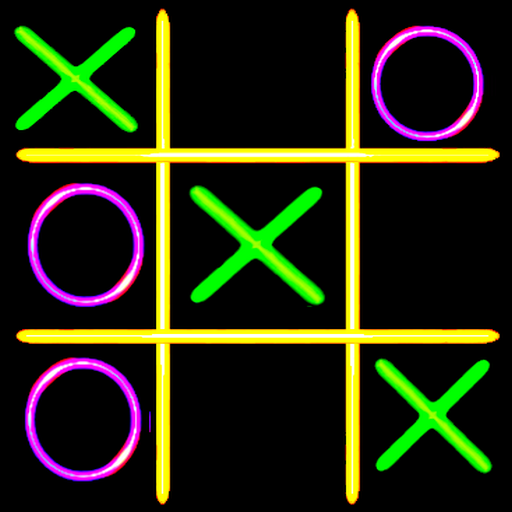
\includegraphics{resources/tic-tac-toe.png}

    \begin{tcolorbox}[breakable, size=fbox, boxrule=1pt, pad at break*=1mm,colback=cellbackground, colframe=cellborder]
\prompt{In}{incolor}{71}{\boxspacing}
\begin{Verbatim}[commandchars=\\\{\}]
\PY{c+cp}{\PYZsh{}}\PY{c+cp}{include} \PY{c+cpf}{\PYZlt{}iostream\PYZgt{}}
\PY{c+cp}{\PYZsh{}}\PY{c+cp}{include} \PY{c+cpf}{\PYZlt{}iomanip\PYZgt{}}
\PY{c+cp}{\PYZsh{}}\PY{c+cp}{include} \PY{c+cpf}{\PYZlt{}string\PYZgt{}}

\PY{k}{using} \PY{k}{namespace} \PY{n+nn}{std}\PY{p}{;}
\end{Verbatim}
\end{tcolorbox}

    \begin{tcolorbox}[breakable, size=fbox, boxrule=1pt, pad at break*=1mm,colback=cellbackground, colframe=cellborder]
\prompt{In}{incolor}{72}{\boxspacing}
\begin{Verbatim}[commandchars=\\\{\}]
\PY{c+c1}{// declare a 2\PYZhy{}d tic\PYZhy{}tac board;}
\PY{c+c1}{// tic\PYZus{}tac\PYZus{}toe[0][0] represents top left box}
\PY{k+kt}{char} \PY{n}{tic\PYZus{}tac\PYZus{}toe}\PY{p}{[}\PY{l+m+mi}{3}\PY{p}{]}\PY{p}{[}\PY{l+m+mi}{3}\PY{p}{]}\PY{p}{;}
\end{Verbatim}
\end{tcolorbox}

    \begin{tcolorbox}[breakable, size=fbox, boxrule=1pt, pad at break*=1mm,colback=cellbackground, colframe=cellborder]
\prompt{In}{incolor}{73}{\boxspacing}
\begin{Verbatim}[commandchars=\\\{\}]
\PY{c+c1}{// define a function to initialize empty tic\PYZus{}tac\PYZus{}toe board}
\PY{c+c1}{// Note: must provide the column\PYZus{}width inside []}
\PY{k+kt}{void} \PY{n+nf}{initTicTacToe}\PY{p}{(}\PY{k+kt}{char} \PY{n}{board}\PY{p}{[}\PY{p}{]}\PY{p}{[}\PY{l+m+mi}{3}\PY{p}{]}\PY{p}{,} \PY{k+kt}{int} \PY{n}{row}\PY{p}{)} \PY{p}{\PYZob{}}
    \PY{k}{for}\PY{p}{(}\PY{k+kt}{int} \PY{n}{i}\PY{o}{=}\PY{l+m+mi}{0}\PY{p}{;} \PY{n}{i}\PY{o}{\PYZlt{}}\PY{n}{row}\PY{p}{;} \PY{n}{i}\PY{o}{+}\PY{o}{+}\PY{p}{)}
        \PY{k}{for}\PY{p}{(}\PY{k+kt}{int} \PY{n}{j}\PY{o}{=}\PY{l+m+mi}{0}\PY{p}{;} \PY{n}{j}\PY{o}{\PYZlt{}}\PY{l+m+mi}{3}\PY{p}{;} \PY{n}{j}\PY{o}{+}\PY{o}{+}\PY{p}{)}
            \PY{n}{board}\PY{p}{[}\PY{n}{i}\PY{p}{]}\PY{p}{[}\PY{n}{j}\PY{p}{]} \PY{o}{=} \PY{l+s+sc}{\PYZsq{}}\PY{l+s+sc}{ }\PY{l+s+sc}{\PYZsq{}}\PY{p}{;} \PY{c+c1}{// space represents empty box}
\PY{p}{\PYZcb{}}
\end{Verbatim}
\end{tcolorbox}

    \begin{tcolorbox}[breakable, size=fbox, boxrule=1pt, pad at break*=1mm,colback=cellbackground, colframe=cellborder]
\prompt{In}{incolor}{74}{\boxspacing}
\begin{Verbatim}[commandchars=\\\{\}]
\PY{k+kt}{void} \PY{n+nf}{printTicTacToe}\PY{p}{(}\PY{k+kt}{char} \PY{n}{board}\PY{p}{[}\PY{p}{]}\PY{p}{[}\PY{l+m+mi}{3}\PY{p}{]}\PY{p}{,} \PY{k+kt}{int} \PY{n}{row}\PY{p}{)} \PY{p}{\PYZob{}}
    \PY{n}{cout} \PY{o}{\PYZlt{}}\PY{o}{\PYZlt{}} \PY{n}{endl} \PY{o}{\PYZlt{}}\PY{o}{\PYZlt{}} \PY{n}{setfill}\PY{p}{(}\PY{l+s+sc}{\PYZsq{}}\PY{l+s+sc}{\PYZhy{}}\PY{l+s+sc}{\PYZsq{}}\PY{p}{)} \PY{o}{\PYZlt{}}\PY{o}{\PYZlt{}} \PY{n}{setw}\PY{p}{(}\PY{l+m+mi}{14}\PY{p}{)} \PY{o}{\PYZlt{}}\PY{o}{\PYZlt{}} \PY{l+s}{\PYZdq{}}\PY{l+s}{ }\PY{l+s}{\PYZdq{}} \PY{o}{\PYZlt{}}\PY{o}{\PYZlt{}} \PY{n}{endl}\PY{p}{;}
    \PY{k}{for}\PY{p}{(}\PY{k+kt}{int} \PY{n}{i}\PY{o}{=}\PY{l+m+mi}{0}\PY{p}{;} \PY{n}{i}\PY{o}{\PYZlt{}}\PY{n}{row}\PY{p}{;} \PY{n}{i}\PY{o}{+}\PY{o}{+}\PY{p}{)} \PY{p}{\PYZob{}}
        \PY{n}{cout} \PY{o}{\PYZlt{}}\PY{o}{\PYZlt{}} \PY{l+s}{\PYZdq{}}\PY{l+s}{| }\PY{l+s}{\PYZdq{}}\PY{p}{;}
        \PY{k}{for}\PY{p}{(}\PY{k+kt}{int} \PY{n}{j}\PY{o}{=}\PY{l+m+mi}{0}\PY{p}{;} \PY{n}{j}\PY{o}{\PYZlt{}}\PY{l+m+mi}{3}\PY{p}{;} \PY{n}{j}\PY{o}{+}\PY{o}{+}\PY{p}{)}
            \PY{n}{cout} \PY{o}{\PYZlt{}}\PY{o}{\PYZlt{}} \PY{n}{tic\PYZus{}tac\PYZus{}toe}\PY{p}{[}\PY{n}{i}\PY{p}{]}\PY{p}{[}\PY{n}{j}\PY{p}{]} \PY{o}{\PYZlt{}}\PY{o}{\PYZlt{}} \PY{l+s}{\PYZdq{}}\PY{l+s}{ | }\PY{l+s}{\PYZdq{}}\PY{p}{;}
        \PY{n}{cout} \PY{o}{\PYZlt{}}\PY{o}{\PYZlt{}} \PY{n}{endl} \PY{o}{\PYZlt{}}\PY{o}{\PYZlt{}} \PY{n}{setfill}\PY{p}{(}\PY{l+s+sc}{\PYZsq{}}\PY{l+s+sc}{\PYZhy{}}\PY{l+s+sc}{\PYZsq{}}\PY{p}{)} \PY{o}{\PYZlt{}}\PY{o}{\PYZlt{}} \PY{n}{setw}\PY{p}{(}\PY{l+m+mi}{14}\PY{p}{)} \PY{o}{\PYZlt{}}\PY{o}{\PYZlt{}} \PY{l+s}{\PYZdq{}}\PY{l+s}{ }\PY{l+s}{\PYZdq{}} \PY{o}{\PYZlt{}}\PY{o}{\PYZlt{}} \PY{n}{endl}\PY{p}{;}
    \PY{p}{\PYZcb{}}
\PY{p}{\PYZcb{}}
\end{Verbatim}
\end{tcolorbox}

    \begin{tcolorbox}[breakable, size=fbox, boxrule=1pt, pad at break*=1mm,colback=cellbackground, colframe=cellborder]
\prompt{In}{incolor}{75}{\boxspacing}
\begin{Verbatim}[commandchars=\\\{\}]
\PY{c+c1}{// let\PYZsq{}s initialize our board}
\PY{n}{initTicTacToe}\PY{p}{(}\PY{n}{tic\PYZus{}tac\PYZus{}toe}\PY{p}{,} \PY{l+m+mi}{3}\PY{p}{)}\PY{p}{;}
\end{Verbatim}
\end{tcolorbox}

    \begin{tcolorbox}[breakable, size=fbox, boxrule=1pt, pad at break*=1mm,colback=cellbackground, colframe=cellborder]
\prompt{In}{incolor}{76}{\boxspacing}
\begin{Verbatim}[commandchars=\\\{\}]
\PY{c+c1}{// let\PYZsq{}s print the empty board}
\PY{n}{printTicTacToe}\PY{p}{(}\PY{n}{tic\PYZus{}tac\PYZus{}toe}\PY{p}{,} \PY{l+m+mi}{3}\PY{p}{)}\PY{p}{;}
\end{Verbatim}
\end{tcolorbox}

    \begin{Verbatim}[commandchars=\\\{\}]

-------------
|   |   |   |
-------------
|   |   |   |
-------------
|   |   |   |
-------------
    \end{Verbatim}

    \begin{tcolorbox}[breakable, size=fbox, boxrule=1pt, pad at break*=1mm,colback=cellbackground, colframe=cellborder]
\prompt{In}{incolor}{77}{\boxspacing}
\begin{Verbatim}[commandchars=\\\{\}]
\PY{c+c1}{// let\PYZsq{}s fill Xs and Os as shown in the above figure}
\PY{c+c1}{// assuming a game play}
\PY{n}{tic\PYZus{}tac\PYZus{}toe}\PY{p}{[}\PY{l+m+mi}{0}\PY{p}{]}\PY{p}{[}\PY{l+m+mi}{0}\PY{p}{]} \PY{o}{=} \PY{l+s+sc}{\PYZsq{}}\PY{l+s+sc}{X}\PY{l+s+sc}{\PYZsq{}}\PY{p}{;}
\PY{n}{tic\PYZus{}tac\PYZus{}toe}\PY{p}{[}\PY{l+m+mi}{0}\PY{p}{]}\PY{p}{[}\PY{l+m+mi}{2}\PY{p}{]} \PY{o}{=} \PY{l+s+sc}{\PYZsq{}}\PY{l+s+sc}{O}\PY{l+s+sc}{\PYZsq{}}\PY{p}{;}
\PY{n}{tic\PYZus{}tac\PYZus{}toe}\PY{p}{[}\PY{l+m+mi}{1}\PY{p}{]}\PY{p}{[}\PY{l+m+mi}{0}\PY{p}{]} \PY{o}{=} \PY{l+s+sc}{\PYZsq{}}\PY{l+s+sc}{O}\PY{l+s+sc}{\PYZsq{}}\PY{p}{;}
\PY{n}{tic\PYZus{}tac\PYZus{}toe}\PY{p}{[}\PY{l+m+mi}{1}\PY{p}{]}\PY{p}{[}\PY{l+m+mi}{1}\PY{p}{]} \PY{o}{=} \PY{l+s+sc}{\PYZsq{}}\PY{l+s+sc}{X}\PY{l+s+sc}{\PYZsq{}}\PY{p}{;}
\PY{n}{tic\PYZus{}tac\PYZus{}toe}\PY{p}{[}\PY{l+m+mi}{2}\PY{p}{]}\PY{p}{[}\PY{l+m+mi}{0}\PY{p}{]} \PY{o}{=} \PY{l+s+sc}{\PYZsq{}}\PY{l+s+sc}{O}\PY{l+s+sc}{\PYZsq{}}\PY{p}{;}
\PY{n}{tic\PYZus{}tac\PYZus{}toe}\PY{p}{[}\PY{l+m+mi}{2}\PY{p}{]}\PY{p}{[}\PY{l+m+mi}{2}\PY{p}{]} \PY{o}{=} \PY{l+s+sc}{\PYZsq{}}\PY{l+s+sc}{X}\PY{l+s+sc}{\PYZsq{}}\PY{p}{;}
\end{Verbatim}
\end{tcolorbox}

    \begin{tcolorbox}[breakable, size=fbox, boxrule=1pt, pad at break*=1mm,colback=cellbackground, colframe=cellborder]
\prompt{In}{incolor}{78}{\boxspacing}
\begin{Verbatim}[commandchars=\\\{\}]
\PY{n}{printTicTacToe}\PY{p}{(}\PY{n}{tic\PYZus{}tac\PYZus{}toe}\PY{p}{,} \PY{l+m+mi}{3}\PY{p}{)}\PY{p}{;}
\end{Verbatim}
\end{tcolorbox}

    \begin{Verbatim}[commandchars=\\\{\}]

-------------
| X |   | O |
-------------
| O | X |   |
-------------
| O |   | X |
-------------
    \end{Verbatim}

    \begin{tcolorbox}[breakable, size=fbox, boxrule=1pt, pad at break*=1mm,colback=cellbackground, colframe=cellborder]
\prompt{In}{incolor}{79}{\boxspacing}
\begin{Verbatim}[commandchars=\\\{\}]
\PY{c+c1}{// let\PYZsq{}s determine winner!}
\PY{k+kt}{char} \PY{n+nf}{findWinner}\PY{p}{(}\PY{k+kt}{char} \PY{n}{board}\PY{p}{[}\PY{p}{]}\PY{p}{[}\PY{l+m+mi}{3}\PY{p}{]}\PY{p}{,} \PY{k+kt}{int} \PY{n}{row}\PY{p}{)} \PY{p}{\PYZob{}}
    \PY{k+kt}{char} \PY{n}{winner}\PY{p}{;} \PY{c+c1}{// is it O or X?}
    \PY{k+kt}{bool} \PY{n}{won}\PY{p}{;}
    \PY{c+c1}{// check 3 rows}
    \PY{k}{for}\PY{p}{(}\PY{k+kt}{int} \PY{n}{i}\PY{o}{=}\PY{l+m+mi}{0}\PY{p}{;} \PY{n}{i}\PY{o}{\PYZlt{}}\PY{n}{row}\PY{p}{;} \PY{n}{i}\PY{o}{+}\PY{o}{+}\PY{p}{)} \PY{p}{\PYZob{}}
        \PY{n}{winner} \PY{o}{=} \PY{n}{board}\PY{p}{[}\PY{n}{i}\PY{p}{]}\PY{p}{[}\PY{l+m+mi}{0}\PY{p}{]}\PY{p}{;} \PY{c+c1}{// whatever symbol is at the first box, that should appear in other columns}
        \PY{n}{won} \PY{o}{=} \PY{n+nb}{true}\PY{p}{;}
        \PY{c+c1}{// check the rest of the columns}
        \PY{k}{for}\PY{p}{(}\PY{k+kt}{int} \PY{n}{j}\PY{o}{=}\PY{l+m+mi}{1}\PY{p}{;} \PY{n}{j}\PY{o}{\PYZlt{}}\PY{l+m+mi}{3}\PY{p}{;} \PY{n}{j}\PY{o}{+}\PY{o}{+}\PY{p}{)} \PY{p}{\PYZob{}}
            \PY{k}{if} \PY{p}{(}\PY{n}{winner} \PY{o}{!}\PY{o}{=} \PY{n}{board}\PY{p}{[}\PY{n}{i}\PY{p}{]}\PY{p}{[}\PY{n}{j}\PY{p}{]}\PY{p}{)} \PY{p}{\PYZob{}}
                \PY{n}{won} \PY{o}{=} \PY{n+nb}{false}\PY{p}{;}
                \PY{k}{break}\PY{p}{;}
            \PY{p}{\PYZcb{}}
        \PY{p}{\PYZcb{}}
        \PY{k}{if} \PY{p}{(}\PY{n}{won}\PY{p}{)} \PY{c+c1}{// we\PYZsq{}ve a winner}
            \PY{k}{return} \PY{n}{winner}\PY{p}{;}
    \PY{p}{\PYZcb{}}
    \PY{c+c1}{// \PYZsh{}FIXME: check columns FIXME\PYZsh{}}
    \PY{c+c1}{// check diagonals }
    \PY{c+c1}{// top left to bottom right}
    \PY{k}{if} \PY{p}{(}\PY{n}{board}\PY{p}{[}\PY{l+m+mi}{0}\PY{p}{]}\PY{p}{[}\PY{l+m+mi}{0}\PY{p}{]} \PY{o}{=}\PY{o}{=} \PY{n}{board}\PY{p}{[}\PY{l+m+mi}{1}\PY{p}{]}\PY{p}{[}\PY{l+m+mi}{1}\PY{p}{]} \PY{o}{\PYZam{}}\PY{o}{\PYZam{}} \PY{n}{board}\PY{p}{[}\PY{l+m+mi}{1}\PY{p}{]}\PY{p}{[}\PY{l+m+mi}{1}\PY{p}{]} \PY{o}{=}\PY{o}{=} \PY{n}{board}\PY{p}{[}\PY{l+m+mi}{2}\PY{p}{]}\PY{p}{[}\PY{l+m+mi}{2}\PY{p}{]}\PY{p}{)} \PY{k}{return} \PY{n}{board}\PY{p}{[}\PY{l+m+mi}{0}\PY{p}{]}\PY{p}{[}\PY{l+m+mi}{0}\PY{p}{]}\PY{p}{;}
    \PY{c+c1}{// \PYZsh{}FIXME: check the other diagonal }
    
    \PY{k}{return} \PY{l+s+sc}{\PYZsq{}}\PY{l+s+sc}{\PYZhy{}}\PY{l+s+sc}{\PYZsq{}}\PY{p}{;} \PY{c+c1}{// return \PYZsq{}\PYZhy{}\PYZsq{} if it\PYZsq{}s a tie}
\PY{p}{\PYZcb{}}
\end{Verbatim}
\end{tcolorbox}

    \begin{tcolorbox}[breakable, size=fbox, boxrule=1pt, pad at break*=1mm,colback=cellbackground, colframe=cellborder]
\prompt{In}{incolor}{80}{\boxspacing}
\begin{Verbatim}[commandchars=\\\{\}]
\PY{k+kt}{char} \PY{n}{winner}\PY{p}{;}
\end{Verbatim}
\end{tcolorbox}

    \begin{tcolorbox}[breakable, size=fbox, boxrule=1pt, pad at break*=1mm,colback=cellbackground, colframe=cellborder]
\prompt{In}{incolor}{81}{\boxspacing}
\begin{Verbatim}[commandchars=\\\{\}]
\PY{n}{winner} \PY{o}{=} \PY{n}{findWinner}\PY{p}{(}\PY{n}{tic\PYZus{}tac\PYZus{}toe}\PY{p}{,} \PY{l+m+mi}{3}\PY{p}{)}\PY{p}{;}
\end{Verbatim}
\end{tcolorbox}

    \begin{tcolorbox}[breakable, size=fbox, boxrule=1pt, pad at break*=1mm,colback=cellbackground, colframe=cellborder]
\prompt{In}{incolor}{82}{\boxspacing}
\begin{Verbatim}[commandchars=\\\{\}]
\PY{k}{if} \PY{p}{(}\PY{n}{winner} \PY{o}{=}\PY{o}{=} \PY{l+s+sc}{\PYZsq{}}\PY{l+s+sc}{\PYZhy{}}\PY{l+s+sc}{\PYZsq{}}\PY{p}{)}
    \PY{n}{cout} \PY{o}{\PYZlt{}}\PY{o}{\PYZlt{}} \PY{l+s}{\PYZdq{}}\PY{l+s}{Oops! it\PYZsq{}s a tie...}\PY{l+s+se}{\PYZbs{}n}\PY{l+s}{\PYZdq{}}\PY{p}{;}
\PY{k}{else}
    \PY{n}{cout} \PY{o}{\PYZlt{}}\PY{o}{\PYZlt{}} \PY{l+s}{\PYZdq{}}\PY{l+s}{Congrats }\PY{l+s}{\PYZdq{}} \PY{o}{\PYZlt{}}\PY{o}{\PYZlt{}} \PY{n}{winner} \PY{o}{\PYZlt{}}\PY{o}{\PYZlt{}} \PY{l+s}{\PYZdq{}}\PY{l+s}{! You win!!}\PY{l+s+se}{\PYZbs{}n}\PY{l+s}{\PYZdq{}}\PY{p}{;}
\end{Verbatim}
\end{tcolorbox}

    \begin{Verbatim}[commandchars=\\\{\}]
Congrats X! You win!!
    \end{Verbatim}

    \hypertarget{labs}{%
\subsection{Labs}\label{labs}}

\begin{enumerate}
\def\labelenumi{\arabic{enumi}.}
\tightlist
\item
  The following lab demonstrates the usage of an array data structure
  and some operations on arrays.

  \begin{itemize}
  \tightlist
  \item
    use partial solution \texttt{array.cpp} in
    \href{./labs/arrays}{labs/arrays} folder
  \item
    use Makefile to compile and debug program
  \item
    fixe all the FIXMEs and write \#FIXED\# next to each FIXME once
    fixed
  \end{itemize}
\end{enumerate}

    \hypertarget{exercises}{%
\subsection{Exercises}\label{exercises}}

\begin{enumerate}
\def\labelenumi{\arabic{enumi}.}
\tightlist
\item
  Write a function that takes an array and finds and returns the max
  value in the array.

  \begin{itemize}
  \tightlist
  \item
    write at least 3 automated test cases
  \end{itemize}
\end{enumerate}

    \begin{tcolorbox}[breakable, size=fbox, boxrule=1pt, pad at break*=1mm,colback=cellbackground, colframe=cellborder]
\prompt{In}{incolor}{83}{\boxspacing}
\begin{Verbatim}[commandchars=\\\{\}]
\PY{c+cp}{\PYZsh{}}\PY{c+cp}{include} \PY{c+cpf}{\PYZlt{}cassert\PYZgt{}}
\end{Verbatim}
\end{tcolorbox}

    \begin{tcolorbox}[breakable, size=fbox, boxrule=1pt, pad at break*=1mm,colback=cellbackground, colframe=cellborder]
\prompt{In}{incolor}{84}{\boxspacing}
\begin{Verbatim}[commandchars=\\\{\}]
\PY{k}{template}\PY{o}{\PYZlt{}}\PY{k}{class} \PY{n+nc}{T}\PY{o}{\PYZgt{}}
\PY{n}{T} \PY{n}{max}\PY{p}{(}\PY{n}{T} \PY{o}{*} \PY{n}{array}\PY{p}{,} \PY{k+kt}{int} \PY{n}{size}\PY{p}{)} \PY{p}{\PYZob{}}
    \PY{n}{assert}\PY{p}{(}\PY{n}{size} \PY{o}{\PYZgt{}}\PY{o}{=} \PY{l+m+mi}{1}\PY{p}{)}\PY{p}{;} \PY{c+c1}{// make sure array is not empty!}
    \PY{n}{T} \PY{n}{curr\PYZus{}max} \PY{o}{=} \PY{n}{array}\PY{p}{[}\PY{l+m+mi}{0}\PY{p}{]}\PY{p}{;}
    \PY{k}{for}\PY{p}{(}\PY{k+kt}{int} \PY{n}{i}\PY{o}{=}\PY{l+m+mi}{1}\PY{p}{;} \PY{n}{i}\PY{o}{\PYZlt{}}\PY{n}{size}\PY{p}{;} \PY{n}{i}\PY{o}{+}\PY{o}{+}\PY{p}{)} \PY{p}{\PYZob{}}
        \PY{c+c1}{// if the value at i is larger than curr\PYZus{}max; update it with the new max}
        \PY{k}{if} \PY{p}{(}\PY{n}{curr\PYZus{}max} \PY{o}{\PYZlt{}} \PY{n}{array}\PY{p}{[}\PY{n}{i}\PY{p}{]}\PY{p}{)}
            \PY{n}{curr\PYZus{}max} \PY{o}{=} \PY{n}{array}\PY{p}{[}\PY{n}{i}\PY{p}{]}\PY{p}{;}
    \PY{p}{\PYZcb{}}
    \PY{k}{return} \PY{n}{curr\PYZus{}max}\PY{p}{;}
\PY{p}{\PYZcb{}}
\end{Verbatim}
\end{tcolorbox}

    \begin{tcolorbox}[breakable, size=fbox, boxrule=1pt, pad at break*=1mm,colback=cellbackground, colframe=cellborder]
\prompt{In}{incolor}{85}{\boxspacing}
\begin{Verbatim}[commandchars=\\\{\}]
\PY{k+kt}{void} \PY{n+nf}{test\PYZus{}max}\PY{p}{(}\PY{p}{)} \PY{p}{\PYZob{}}
    \PY{n}{assert}\PY{p}{(}\PY{n}{max}\PY{p}{(}\PY{p}{\PYZob{}}\PY{l+m+mi}{1}\PY{p}{,} \PY{l+m+mi}{2}\PY{p}{,} \PY{l+m+mi}{3}\PY{p}{\PYZcb{}} \PY{o}{=}\PY{o}{=} \PY{l+m+mi}{3}\PY{p}{)}\PY{p}{)}\PY{p}{;}
    \PY{n}{assert}\PY{p}{(}\PY{n}{max}\PY{p}{(}\PY{p}{\PYZob{}}\PY{l+m+mi}{10}\PY{p}{,} \PY{l+m+mi}{\PYZhy{}5}\PY{p}{,} \PY{l+m+mi}{\PYZhy{}30}\PY{p}{\PYZcb{}} \PY{o}{=}\PY{o}{=} \PY{l+m+mi}{10}\PY{p}{)}\PY{p}{)}\PY{p}{;}
    \PY{n}{assert}\PY{p}{(}\PY{n}{max}\PY{p}{(}\PY{p}{\PYZob{}}\PY{l+m+mi}{\PYZhy{}10}\PY{p}{,} \PY{l+m+mi}{\PYZhy{}5}\PY{p}{,} \PY{l+m+mi}{\PYZhy{}30}\PY{p}{,} \PY{l+m+mi}{0}\PY{p}{,} \PY{l+m+mi}{\PYZhy{}100}\PY{p}{\PYZcb{}} \PY{o}{=}\PY{o}{=} \PY{l+m+mi}{0}\PY{p}{)}\PY{p}{)}\PY{p}{;}
    \PY{n}{cerr} \PY{o}{\PYZlt{}}\PY{o}{\PYZlt{}} \PY{l+s}{\PYZdq{}}\PY{l+s}{all test cases passed for max()}\PY{l+s+se}{\PYZbs{}n}\PY{l+s}{\PYZdq{}}\PY{p}{;}
\PY{p}{\PYZcb{}}
\end{Verbatim}
\end{tcolorbox}

    \begin{tcolorbox}[breakable, size=fbox, boxrule=1pt, pad at break*=1mm,colback=cellbackground, colframe=cellborder]
\prompt{In}{incolor}{86}{\boxspacing}
\begin{Verbatim}[commandchars=\\\{\}]
\PY{n}{test\PYZus{}max}\PY{p}{(}\PY{p}{)}\PY{p}{;}
\end{Verbatim}
\end{tcolorbox}

    \begin{Verbatim}[commandchars=\\\{\}]
all test cases passed for max()
    \end{Verbatim}

    \begin{enumerate}
\def\labelenumi{\arabic{enumi}.}
\setcounter{enumi}{1}
\tightlist
\item
  Write a function that takes an array and finds and returns the min
  value in the array.

  \begin{itemize}
  \tightlist
  \item
    write at least 3 automated test cases
  \end{itemize}
\item
  Write a complete C++ program that computes some statistical values on
  any given number of numbers

  \begin{itemize}
  \tightlist
  \item
    prompt user to enter a bunch of numbers
  \item
    find and display the max and min values
  \item
    find and display the average or mean
  \item
    find and print the range (max - min) in the array
  \item
    find and display the mode or modal (the number with largest
    frequency)
  \item
    program continues to run until the user wants to quit
  \end{itemize}
\item
  Write a search function that checks if a given value is found in an
  array.

  \begin{itemize}
  \tightlist
  \item
    write 3 automated test cases
  \end{itemize}
\end{enumerate}

    \hypertarget{kattis-problems}{%
\subsection{Kattis problems}\label{kattis-problems}}

\begin{itemize}
\tightlist
\item
  a large number of difficult problems require to store data in 1 or 2-d
  arrays and manipulate the data
\item
  solve the following Kattis problems writing at least 3 automated test
  cases for each function used as part of the solution
\end{itemize}

\begin{enumerate}
\def\labelenumi{\arabic{enumi}.}
\item
  Falling Apart - https://open.kattis.com/problems/fallingapart
\item
  Statistics - https://open.kattis.com/problems/statistics
\item
  Line Them Up - https://open.kattis.com/problems/lineup
\end{enumerate}

    \hypertarget{summary}{%
\subsection{Summary}\label{summary}}

\begin{itemize}
\tightlist
\item
  learned about array and types of arrays
\item
  passing array to functions
\item
  similarity between array and pointers in terms of using memory
  addressses
\item
  methods or member functions or lack there of
\item
  array of C++ strings and C-strings
\item
  went over a quick intro to buffer overflow security vulnerability
\item
  sorting using \textless algorithm\textgreater{} and writing our own
  bubble sort
\item
  2-d array and it's application on tic-tac-toe game
\end{itemize}

    \begin{tcolorbox}[breakable, size=fbox, boxrule=1pt, pad at break*=1mm,colback=cellbackground, colframe=cellborder]
\prompt{In}{incolor}{ }{\boxspacing}
\begin{Verbatim}[commandchars=\\\{\}]

\end{Verbatim}
\end{tcolorbox}


    % Add a bibliography block to the postdoc
    
    
    
\end{document}
